\documentclass[a4paper,12pt]{report}

\usepackage[utf8]{inputenc}
\usepackage[T1]{fontenc}
\usepackage{array}
\usepackage{amsmath}
\usepackage[english]{babel}
\usepackage{bm}
\usepackage{graphicx}
\usepackage[a4paper]{geometry}
\usepackage[colorlinks=true,urlcolor=blue,linkcolor=blue]{hyperref}
\usepackage{url}
\usepackage[nottoc,numbib]{tocbibind}
\usepackage{color}
\usepackage{epstopdf}
\usepackage{xcolor}
\usepackage[backend=biber,style=phys]{biblatex}
\usepackage{upgreek}
\usepackage[capbesideposition={right,center}]{floatrow}
\usepackage[ampersand]{easylist}

\addbibresource{../Bibliography.bib}

\makeatletter
	\renewcommand{\thechapter}{\Roman{chapter}}
\makeatother

\newcolumntype{M}[1]{>{\centering\arraybackslash}m{#1}}

\floatsetup[table]{style=plaintop}

\begin{document}

\chapter{Diluted magnetic semiconductor quantum dots\label{DMSQDTh}}

%Plan général :
%	I - Les QD
%		- On commence avec la decription général des semi-conducteurs
%		- On étudie leur structure de bande à k = 0
%		- On veut voir comment ça évolue autour de k = 0 -> k.p method (problème pour les trous lourd) puis Luttinger hamiltonian
%		- On a du CdTe sur ZnTe -> lattice parameters different -> strain -> BP hamiltonian
%		- On réduit la symmétrie -> QD et confinement des porteurs
%		- Interaction entre porteurs -> Coulomb et l'interation d'échange
%		- Effet de l'anisotropie des contraintes ou de la boîte -> la VBM
%	II - Les DMS
%		- Cas général : insertion d'une faible densité d'atome magnétique dans les semi-conducteurs, interaction d'échange entre porteurs du SC et ceux de l'atome magnétique. Mise en place du hamiltonien pour cet interaction sous forme d'un hamiltonien d'Heisenberg H = I \sigma.S.
%		- Cas particulier : Mn, GS loin dans la bande de valence.
%		- Cas particulier : Cr, GS proche du sommet de la bande de valence.
%	III - Mag at dans lattice
%		- Mn : effet du réseau sur ses niveaux
%		- Cr : effet du réseau sur ses niveaux
%	IV - Illustration : le X-Mn
%		- Simple modèle : ne prend pas en compte les effets de VBM oudu SO sur les niveaux de spins de l'atome de Mn.
% 		- Carrier as effective magnetic -> split des niveaux du Mn
%		- Systèe symmétrique pour une inversion de l'axe z -> niveau de spin du Mn dégénéré deux à deux avec spins Mn opposés et spin electron opposé
%		- Spectre obtenu en micro-photoluminescence = photographie de l'état statistique du Mn

	This chapter aims to present the system we will study as well as the main theoretical tools one needs to understand it. We begin presenting the semiconductor physics, and especially the CdTe crystal and electronic structure, and the interaction between carriers and light. We then see how the strains affect the energy levels of the carriers. We then reduce the dimensions of the system, confining the carriers in three dimension, creating what is called the quantum dots (QDs). We describe the effect of the confinement on the carriers, before explaining  how they interact with each other inside the QD. We finish the section with the effect of the shape and strains anisotropy on the carriers and the emission of the QDs.
	
	In the second section, we introduce the magnetic atoms and see how they interact with the semiconductor carriers. We begin describing the interaction between localized electrons on the outer shell of a magnetic atom, and carriers of interest in the semiconductor. We then apply this description to the two magnetic atoms of this thesis: Manganese (Mn) and Chromium (Cr).
	
	In the third section, it is shown how the insertion of the magnetic atom in the semiconductor matrix affects its spin. We begin by describing the case of the Mn, weakly coupled to the crystal field. We continue with the case of Cr, which is strongly affected by the crystal field and its modification by the strains.
	
	We finish this chapter by applying the different concepts we described so far to a simple system: an exciton coupled to a Mn atom in a neutral quantum dot.
	
%	In the next sections, we open the discussion on the magnetic atoms, starting with the Diluted Magnetic Semiconductors, semiconductors with a low density of magnetic impurity inserted in the lattice. We see how these impurities can dramatically change the behaviour of the carriers and thus the properties of said semiconductor. We then give more details on the two atoms we focus on in this thesis: the Manganese and the Chromium. The second section details their interactions with the carriers, while we study in the third their interaction with the semiconductor crystal field.
%	
%	Finally, we give a simple example of application for these theories, studying a simple system: an exciton and a single Manganese atom in a quantum dot.

	\section{II-VI semiconductor quantum dots}
	
	
%Plan:
% - Semicon at k = 0 + selection rule
% - Semicon at k =/= 0
% - Effect of confinement on isolated carrier
% - Coulomb interaction between electron and hole (CB and VB)
%		-> BP separate the hamiltonian of a single electron in CB ineracting with the one in VB in two term: direct and exchange
%		-> Direct interaction, introduce exciton (attractive direct), charged exciton and biexciton
%		-> Short range exchange: introduce $\delta_0$ and $\delta_2$
%		-> Long range exchange: introduce $\delta_1$ and $\varphi_1$
	
 		\subsection{Band structure of CdTe and ZnTe\label{BandStruct}}
		
		CdTe and ZnTe are II-VI semiconductors, meaning they are composed of an anion from the column VI of periodic table (Te), and a cation from the column II (Cd or Zn). They both naturally crystallize in a zinc blend structure when grown in Molecular Beam Epitaxy (MBE, see  Chap.~II%~\ref{Growth}
 for more informations on this technique). As shown in Fig.~\ref{Zinc-Blende} (a), in this structure, each species is organized in a face centered lattice, one of them being shifted from the other by a quarter of the [111] diagonal. Each ion is then in a tetragonal environment. In other words, the zinc-blende structure is of the $T_d$ space-group.

	\begin{figure}[h!]
	\caption{(a) Zinc-blende crystal elementary cell. Both CdTe and ZnTe crystallize in this structure. (b) Bonding and anti-bonding state arising from the hybridization of $s$ and $p$ orbitals.\label{Zinc-Blende}}
	{\begin{center}
		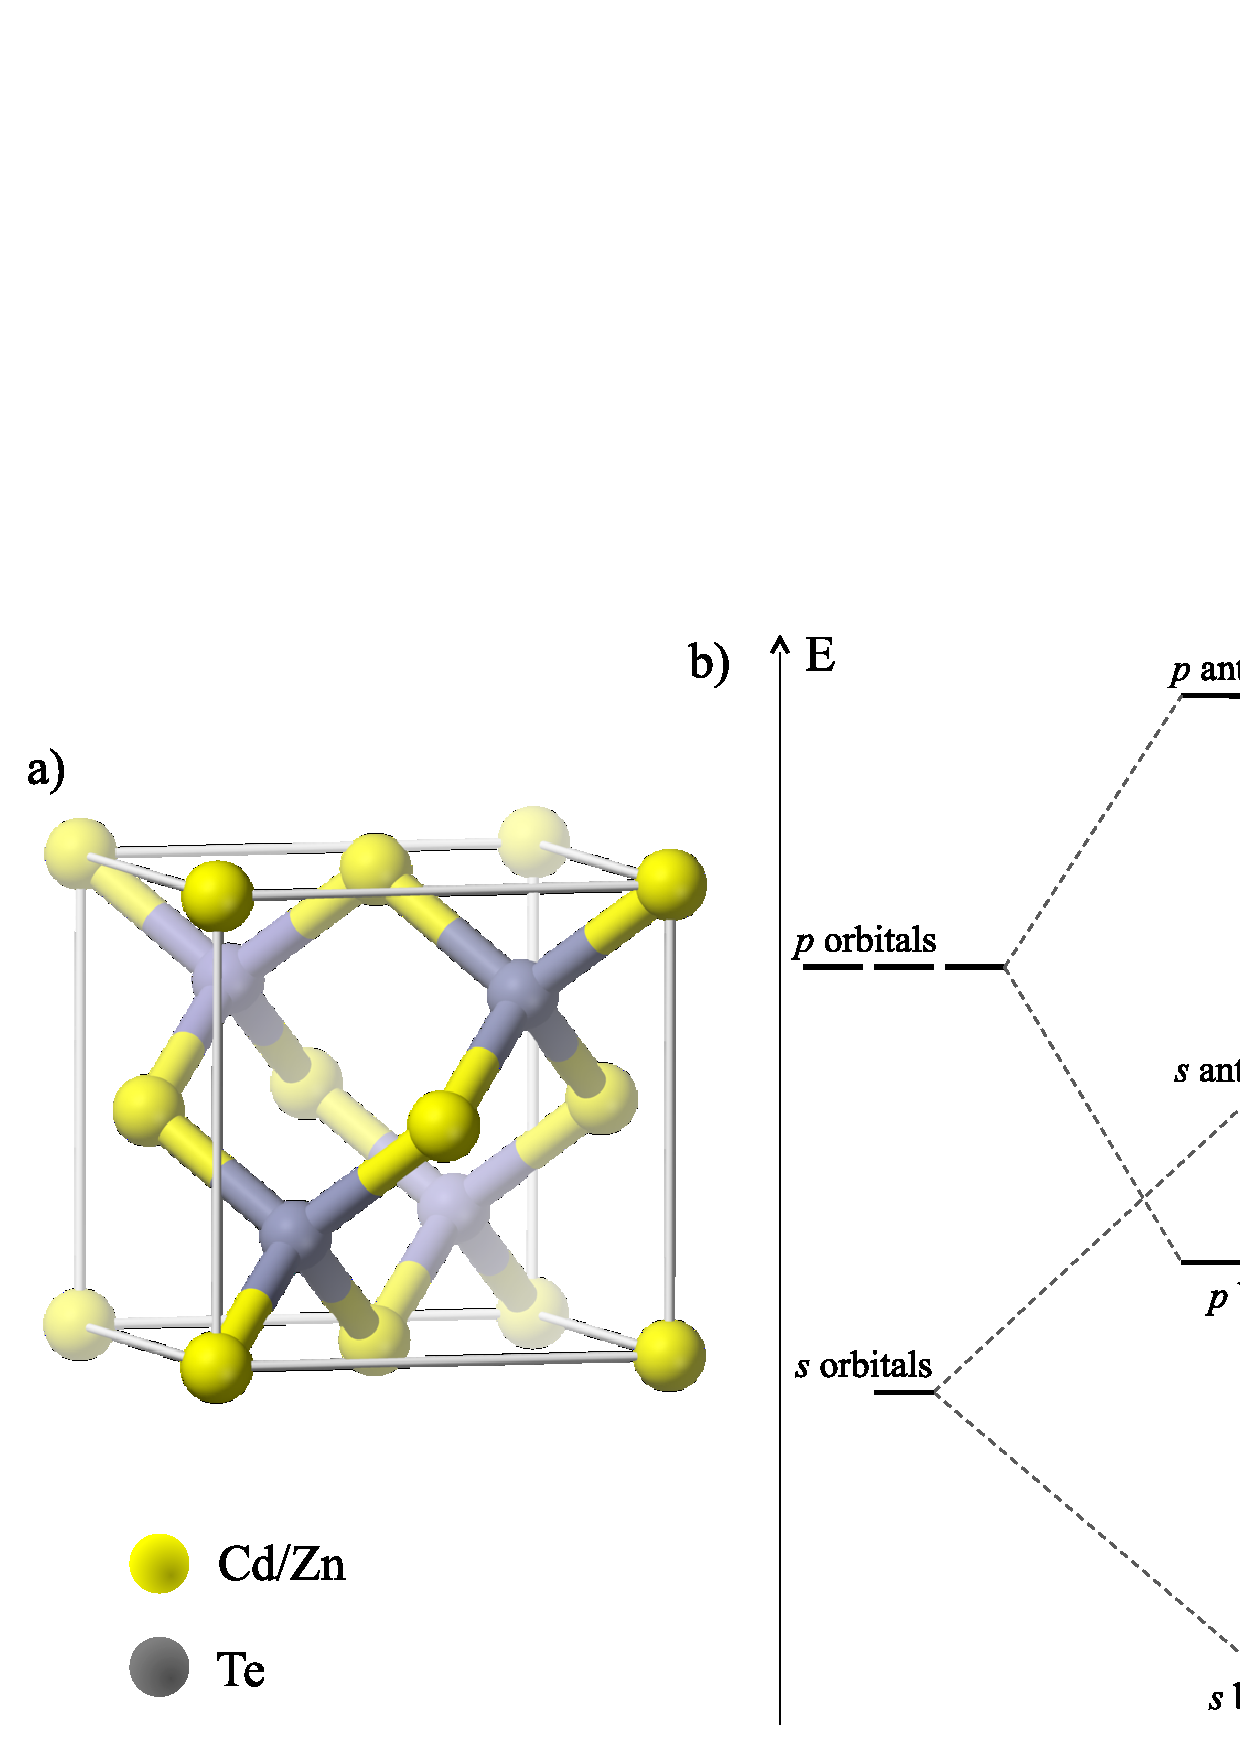
\includegraphics[width=13cm]{Pictures/CrystalAndHybridization.png}
	\end{center}}
	\end{figure}

	The external orbitals for the cation are $s$ (4$d^{10}$5$s^2$ for Cd,  3$d^{10}$4$s^2$ for Zn) and $p$ for the anion (4$d^{10}$5$s^2$5$p^4$ for Te). In the crystal, their orbitals hybridize to form the conduction band and the valence band of the semiconductor. A good and more simple picture of this construction can be given considering the hybridization of two elements of the column IV of the periodic table. It is the well-known $sp$-hybridization. A single unit of the crystal contains 8 valence electrons, coming from the $s$ and $p$ levels of the ions. The $s$ and $p$ orbitals of these atoms hybridize to form 8 levels, 4 bonding and 4 anti-bonding.
	
	The lowest band of the bonding levels, coming from $s$ orbitals, will be filled by 2 valence electrons. 6 will be taken to fill the three bonding bands of higher energy, formed by the hybridization of $p$ orbitals. Those bonding states form the valence band. At higher energy, the anti-bonding states form the conduction band. Since all the available electrons are used to fill the valence band, the conduction band is empty in the ground state. The lower energy band of the conduction band is formed by the anti-symmetric combination of the $s$ orbitals. At higher energy, the anti-symmetric hybridization of $p$ orbitals form three other bands.

	The energy needed to excite one electron from the higher energy state of the valence band to the lower energy state of the conduction band is called the gap. The gap is really important for the opto-electric properties of the semiconductor. In the ZnTe and CdTe cases, they are equal to $E_{g, ZnTe} = 2.40$ eV and  $E_{g, CdTe} = 1.60$ eV at 5K~\cite{FurdynaDMS}.
	
	The promotion of an electron to the conduction band leave in the valence band a quasi-particule called a hole. The hole represents the absence of an electron, and has thus the opposite characteristic (spin, charge, wave vector...) as the missing electron. Aside from the promotion of an electron to the conduction band, holes can also be injected in the semiconductor via the introduction of p-type defect.
	
	\begin{figure}[h!]
	\caption{Different type of heterojunctions between two semiconductors.\label{SCType}}
	{\begin{center}
		\includegraphics[width=14cm]{Pictures/SCType.png}
	\end{center}}
	\end{figure}	
	
	When growing two semiconductors of different band gap on top of each other, a band offset appears at the interface. This offset is distributed between the valence band and the conduction band. It can be distributed in three different ways, depending of the relative energies of the conductions bands and valence bands. Those configurations are illustrated in Fig.~\ref{SCType}. CdTe grown over ZnTe is a type I semiconductor. In this case, both the electrons and the holes are confined in the semiconductor of smaller gap (since holes have the opposite energies as the missing electrons, they are confined in the higher energy part of the valence band). For CdTe on ZnTe, the valence band offset is of about 0.1 meV, about 5\% of the total offset~\cite{VBOZnTeCdTe}. The conduction band then takes most of the band gap offset. The confinement of the electrons in the conduction band is thus far more efficient than confinement of the hole.
	
		\subsubsection*{Band structure near the center of the Brillouin zone ($k = 0$)\label{k0Descr}}
			
	The optical properties of direct gap semiconductors such as CdTe and ZnTe are controlled by their symmetry at the center of the Brillouin zone, corresponding to an electron wave vector $\mathbf{k} = 0$. At this point, the conduction band has the $T_d$ group $\Gamma_6$ symmetry. As discussed, this band comes from the overlap of atomic $s$ orbitals, meaning the conduction electron will have no orbital momentum, and a total angular momentum $J = \dfrac{1}{2}$.
	
	The valence band is formed from $p$ orbitals, presenting a orbital momentum $L = 1$. It couples at $k = 0$ with the electron spin $S = 3/2$ through the spin-orbit coupling. $\mathbf{L}$ and $\mathbf{S}$ are then not good quantum number anymore. We can show that $\mathbf{J} = \mathbf{L}+ \mathbf{S}$, however, commute the hamiltonian presented in the following sections. This composition gives two sub-bands of total angular momentum $J = 1/2$ and $J = 3/2$. In the $T_d$ group, the quadruplet $J = 3/2$ is of $\Gamma_8$ symmetry, and the doublet $J = 1/2$ is of $\Gamma_7$ symmetry. Those bands are split by the spin-orbit interaction, with an energy $\Delta_{SO}$. The eigenstates $J^2$, $J_z$ are chosen as a basis for the system at $k = 0$.
	
	The conduction band and valence band states can now be written from the composition of the two uncoupled basis:
	\begin{align}	
		\Gamma_6&:
			\label{eBasis}
			\def\arraystretch{2.0}
			\begin{array}{lll}
				u_{\Gamma_6, \frac{1}{2}} &= |\dfrac{1}{2}, \dfrac{1}{2}\rangle &= |S\rangle|\uparrow\rangle \\
				u_{\Gamma_6, -\frac{1}{2}} &= |\dfrac{1}{2}, -\dfrac{1}{2}\rangle &= |S\rangle|\downarrow\rangle
			\end{array}
	\end{align}
	\begin{align}
		\Gamma_8&:
			\label{hBasis}
			\def\arraystretch{2.0}
			\begin{array}{lll}
				u_{\Gamma_8, \frac{3}{2}} &= |\dfrac{3}{2}, \dfrac{3}{2}\rangle &= |1\rangle|\uparrow\rangle \\
				u_{\Gamma_8, \frac{1}{2}} &= |\dfrac{3}{2}, \dfrac{1}{2}\rangle &= \sqrt{\dfrac{2}{3}}|0\rangle|\uparrow\rangle + \sqrt{\dfrac{1}{3}}|1\rangle|\downarrow\rangle \\	
				u_{\Gamma_8, -\frac{1}{2}} &= |\dfrac{3}{2}, -\dfrac{1}{2}\rangle &= \sqrt{\dfrac{2}{3}}|0\rangle|\downarrow\rangle + \sqrt{\dfrac{1}{3}}|1\rangle|\uparrow\rangle \\	
				u_{\Gamma_8, -\frac{3}{2}} &= |\dfrac{3}{2}, -\dfrac{3}{2}\rangle &= |-1\rangle|\downarrow\rangle \\	
			\end{array} \\
		\nonumber \\
		\Gamma_7&:
			\def\arraystretch{2.0}
			\begin{array}{ll}
				|\dfrac{1}{2}, \dfrac{1}{2}\rangle &= \sqrt{\dfrac{2}{3}}|1\rangle|\downarrow\rangle - \sqrt{\dfrac{1}{3}}|0\rangle|\uparrow\rangle \\
				|\dfrac{1}{2}, -\dfrac{1}{2}\rangle &= -\sqrt{\dfrac{2}{3}}|-1\rangle|\uparrow\rangle + \sqrt{\dfrac{1}{3}}|0\rangle|\downarrow\rangle
			\end{array}
	\end{align}
with:
	\begin{align*}
		|1\rangle &= -\frac{|X\rangle + i |Y\rangle}{\sqrt{2}} \\
		|0\rangle &= |Z\rangle \\
		|-1\rangle &= \frac{|X\rangle - i |Y\rangle}{\sqrt{2}}
	\end{align*}
where $|X\rangle$, $|Y\rangle$ and $|X\rangle$ are the wave function of the valence band top at $k = 0$. They are calculated from the hybridization of the atomic orbital $p_X$, $p_Y$ and $p_Z$.

%	Introducing the spin-orbit interaction, the conduction band, formed by the hybridization of $s$ orbitals, is of $\Gamma_6$ (spherical) symmetry at the center of the Brillouin zone (for $k \simeq 0$), two-fold degenerated, with an orbital momentum (spin) $\sigma = \dfrac{1}{2}$. In a similar fashion, the valence band will be split into two bands: a first one of $\Gamma_8$ symmetry, with a spin $J = \dfrac{3}{2}$, four-fold degenerated ; and the second one, at lower energy, of $\Gamma_7$ symmetry, with a spin $\dfrac{1}{2}$, two-fold degenerated. The splitting $\Gamma_7-\Gamma_8$ is of $\Delta_{SO} \simeq 0.9$ eV in II-VI semiconductor. This gap is wide enough to ignore the effect of the $\Gamma_7$ band for the rest of this document and focusing on the effect between the top of the valence band and the bottom of the conduction band.
	
		Since $\Delta_{SO} \simeq 0.9$ eV for CdTe and ZnTe, the $\Gamma_7$ band is far enough in the valence band to be able to limit our study to the interaction between the $\Gamma_6$ and $\Gamma_8$ bands. The electrons in the conduction band have a spin $\sigma = \frac{1}{2}$. The spin operator can therefore be written using the Pauli matrices. For a quantization along the growth axis of the semiconductor, noted $z$:
	\begin{align}
			\sigma_x = \dfrac{1}{2}
						\begin{pmatrix}
							0 & 1 \\
							1 & 0
						\end{pmatrix} \qquad ; \qquad
			\sigma_y = \dfrac{1}{2}
						\begin{pmatrix}
							0 & -i \\
							i & 0
						\end{pmatrix} \qquad ; \qquad
			\sigma_z = \dfrac{1}{2}
						\begin{pmatrix}
							1 & 0 \\
							0 & -1
						\end{pmatrix}
	\end{align}
In the same way, we can define the operators at the top of the valence band. For an angular momentum $J = \frac{3}{2}$ quantized along the $z$ axis, we have in the basis $(3/2, 1/2, -1/2, -3/2)$:
	\begin{align}
		\label{holeAngMom}
		\begin{array}{ccl}
			J_x = \begin{pmatrix}
						0 & \frac{\sqrt{3}}{2} & 0 & 0 \\
						\frac{\sqrt{3}}{2} & 0 & 1 & 0 \\
						0 & 1 & 0 & \frac{\sqrt{3}}{2} \\
						0 & 0 & \frac{\sqrt{3}}{2} & 0
					\end{pmatrix} & ; &
			J_y = i\begin{pmatrix}
						0 & -\frac{\sqrt{3}}{2} & 0 & 0 \\
						\frac{\sqrt{3}}{2} & 0 & -1 & 0 \\
						0 & 1 & 0 & -\frac{\sqrt{3}}{2} \\
						0 & 0 & \frac{\sqrt{3}}{2} & 0
					\end{pmatrix}
		\end{array} \nonumber \\
		 J_z = \begin{pmatrix}
						\frac{3}{2} & 0 & 0 & 0 \\
						0 & \frac{1}{2} & 0 & 0 \\
						0 & 0 & -\frac{1}{2} & 0 \\
						0 & 0 & 0 & -\frac{3}{2}
					\end{pmatrix} \qquad \qquad \qquad \qquad \quad \; \;
	\end{align}

Finally, for any spin operator $O$ ($O = \bm{\upsigma}$, $\mathbf{J}$ or any other angular momentum operator of this document), we can define the ladder operator, flipping the considered spin by one unit, such as $O_+|O\rangle \propto |O+1\rangle$ and $O_-|O\rangle \propto |O-1\rangle$. They read in the general case as:
	\begin{align}
		O_+ = O_x + iO_y \\
		O_- = O_x - iO_y
	\end{align}

	We are mainly interested in two light matter interaction in the semiconductor:  absorption of a photon of energy equal to or higher than the band gap by an electron of the valence band to reach the conduction band; or emission of photon by an electron relaxing from the conduction band to the valence band. However, angular momentum conservation rules forbid some transitions. In order to find them, we consider the coupling between a conduction band electron $|\Psi_c\rangle$ and a valence band hole $|\Psi_v\rangle$ through, in the dipolar approximation, the hamiltonian ${\cal H}_{dip} = -\mathbf{d}.\mathbf{E}$ with $\mathbf{d}$ the dipole operator and $\mathbf{E}$ the electric field, that can also be written ${\cal H}_{dip} = -\frac{e}{m}\mathbf{p}.\mathbf{A}$ with $\mathbf{p}$ the electron momentum and $\mathbf{A}$ the potential vector~\cite{RosencherOptoElec}. In this section, we go with the later. We then get:
	\begin{align}
		\langle \Psi_v | {\cal H}_{AF} | \Psi_c \rangle \propto \langle u_{\Gamma_8, J_z} | \mathbf{p} | u_{\Gamma_6, \sigma_z} \rangle
	\end{align}
Considering that $|\uparrow\rangle$ and $|\downarrow\rangle$ are orthogonal states, we can easily deduce the authorized transitions:
	\begin{easylist}[itemize]
		& Between $| u_{\Gamma_6, +\frac{1}{2}} \rangle$ and $| u_{\Gamma_8, +\frac{3}{2}} \rangle$ (corresponding to a hole $J_z = -\frac{3}{2}$), coupled by $p_- = p_x - ip_y$, corresponding to a $\sigma-$ photon absorption or emission.
		& Between $| u_{\Gamma_6, -\frac{1}{2}} \rangle$ and $| u_{\Gamma_8, -\frac{3}{2}} \rangle$ (corresponding to a hole $J_z = +\frac{3}{2}$), coupled by $p_+ = p_x + ip_y$, corresponding to a $\sigma+$ photon absorption or emission.
		& Between $| u_{\Gamma_6, +\frac{1}{2}} \rangle$ and $| u_{\Gamma_8, -\frac{1}{2}} \rangle$ (corresponding to a hole $J_z = +\frac{1}{2}$) coupled via a $\sigma+$ photon absorption or emission.
		& Between $| u_{\Gamma_6, -\frac{1}{2}} \rangle$ and $| u_{\Gamma_8, +\frac{1}{2}} \rangle$ (corresponding to a hole $J_z = -\frac{1}{2}$) coupled via a $\sigma-$ photon absorption or emission.
		& Between $| u_{\Gamma_6, \pm\frac{1}{2}} \rangle$ and $| u_{\Gamma_8, \mp\frac{1}{2}} \rangle$ coupled via a $\pi_z$ photon absorption or emission.
	\end{easylist}
Those transitions are summarize on Fig.~\ref{SelectionRules}, with their respective relative probability calculated from the oscillator strength of each of these transitions.

	\begin{figure}[h!]
	\begin{center}
		\includegraphics[width=14.8cm]{Pictures/SelectionRules.eps}
	\end{center}
	\caption{Selection rules for optical transitions between valence band and conduction band in a quantum well. They are presented in this confined environment in order to have a clear separation between the heavy holes ($J_z = \pm \frac{3}{2}$) and the light holes ($J_z = \pm \frac{1}{2}$). Circularly polarized transition are noted $\sigma\pm$ and $\pi_z$ stands for a linear polarization along $z$ axis.}
	\label{SelectionRules}
	\end{figure}

%	Exciton of total angular momentum $J_z = \pm2$ also exists. They are formed by an electron of spin $\pm \dfrac{1}{2}$ coupled to a hole of spin $\pm \dfrac{3}{2}$. However, since this transition is forbidden by the conversation of angular momentum, they cannot recombine radiatively.

		\subsubsection*{$k \neq 0$: the $\mathbf{k}.\mathbf{p}$ approach}	
	
	The whole CdTe band structure is presented on Fig.~\ref{BandStruct}. We see that the maximum of the valence band and the minimum of the conduction band are both reached at the point $\Gamma$, center of Brillouin zone, corresponding to an electron wave vector $\mathbf{k} = 0$. This is characteristic of a direct band gap semiconductor. 
	
	Near this band edge, we can describe the curvature of the energy $E(\mathbf{k})$ of the band using an effective mass for the carrier on it:
	\begin{align}
		E_{\{c,v\}} (\mathbf{k}) = - \frac{(\hbar k)^2}{2m_{\{c,v\}}(\mathbf{k})}
	\end{align}		
	 As we move away from the $\Gamma$ point, the valence band split into two branches: the one with small curvature, meaning a high effective mass for the carriers on it, is called the heavy-hole (hh) band, while the one presenting the highest curvature and smallest effective mass is called the light-hole (lh) band.
	 
	\begin{figure}[h!]
	\begin{center}
		\includegraphics[width=11.5cm]{Pictures/CdTeband.eps}
	\end{center}
	\caption{CdTe band structure}
	\label{BandStruct}
	\end{figure}

	One way to understand this evolution is to apply the $\mathbf{k}.\mathbf{p}$ approximation, as proposed by Kane in 1957~\cite{KaneBandkp}. This model gives an estimation of the electronic band structure starting from the exact solution of the Schrödinger equation at the center of the Brillouin. The hamiltonian to resolve is then :	
	\begin{align}
		\label{SchrödEq}
		\left(\frac{p^2}{2m_0} + U(\mathbf{r})\right)|\psi_{n,\mathbf{k}}\rangle = E_{n,\mathbf{k}} |\psi_{n,\mathbf{k}}\rangle
	\end{align}
with $n$ the band index, $\mathbf{p} = -i\hbar\mathbf{\nabla}$, $U(\mathbf{r})$ the potential of the crystal, $m_0$ the mass of a free carrier and $|\psi_{n,\mathbf{k}}\rangle$ the Bloch wave, separated between a periodic part $u_{n,\mathbf{k}} (\mathbf{r})$ and plane-wave part $\exp(i\mathbf{k}.\mathbf{r})$ as follow:
	\begin{align}
		|\psi_{n,\mathbf{k}}\rangle = u_{n,\mathbf{k}} (\mathbf{r}) \exp (i\mathbf{k}.\mathbf{r})\label{BlochWave}
	\end{align}
Using Eq.~\ref{BlochWave} and after development of the gradient of $\psi_{n, \mathbf{k}}$, it is possible to rewrite Eq.~\ref{SchrödEq} as a function of the periodic part only:
	\begin{align}
		\label{kpHamil}
		\left(\frac{p^2}{2m_0} + U(\mathbf{r}) + \frac{\hbar^2 k^2}{2m_0} + \frac{\hbar}{m_0}\mathbf{k}.\mathbf{p}\right)u_{n,\mathbf{k}} = E_{n,\mathbf{k}} u_{n,\mathbf{k}}
	\end{align}
	
	To find the solutions around $k = 0$, we develop the $u_{n,\mathbf{k}}$ on the basis of the $\{u_{n,0}\}_n$ as:
	\begin{align*}
		u_{n,\mathbf{k}} = \sum_{n'} c_{n'} u_{n',0}
	\end{align*}
Assuming that the $u_{n,0}$ are known, we can calculate the matrix elements of Eq.~\ref{kpHamil}.
%Since the $\{u_{n,0}\}_n$ basis is infinite, we have to limit our study to a certain number of $n$. In his original work, Kane did the calculation with 8 bands. A simple illustration is often done with only 2 bands, the $\Gamma_6$ and $\Gamma_8$ ones, and gives the energies:
The resolution of this hamiltonian is often done in the books~\cite{kpMethod}, and gives, taking into account the $\Gamma_6$ and $\Gamma_8$ bands only:
%	We solve this hamiltonian for carrier on the $\Gamma_6$ and $\Gamma_8$ bands. The $z$-axis is defined along the growth direction of the semiconductor and chosen as the quantization axis. The resolution was done in detail in Claire Le Gall PhD thesis~\cite{ClaireTh}. We then find the energies:
	\begin{align}
		\begin{array}{l}
		E_c (k_z) = E_c + \dfrac{\hbar^2 k_z^2}{2m_c} \\
		E_{v, \pm\frac{1}{2}} (k_z) = E_v - \dfrac{\hbar^2 k_z^2}{2m_{lh}} \\
		E_{v, \pm\frac{3}{2}} (k_z) = E_v + \dfrac{\hbar^2 k^2_z}{2m_{0}}
		\end{array}	
	\end{align}
with $E_c$ (respectively, $E_v$) the energy of the conduction band (respectively, the valence band), $m_c$ the effective mass of the carrier in the conduction band and $m_{lh}$ the effective mass of the light hole. One can see that the splitting of the valence band separate the carrier with a spin $J_z = \pm \frac{3}{2}$ (hh) from the one with a spin $J_z = \pm \frac{1}{2}$ (lh). However, the hh presents a positive curvature in this results, meaning a positive effective mass. This contradict the schema given on Fig.~\ref{BandStruct}. Taking into account the coupling with the higher energy band, hh are found to have indeed a negative curvature~\cite{kpMethod}. Considering only two bands is too rough to really model the system.

		\subsubsection*{$k \neq 0$: the Luttinger hamiltonian}

	Another way to obtain the matrix describing the $\Gamma_8$ band is to use symmetry consideration. Luttinger showed in 1956~\cite{LuttingerHam} that the only Hamiltonian fulfilling the cubic symmetry is:
	\begin{align}
	\label{LuttHamil}
		{\cal H}_L = - \frac{h^2}{2m_0}\left(\gamma_1 k^2 I_4 - 2 \gamma_2 \sum_i k_i^2 \left(J_i^2 - \frac{1}{3} J^2\right) - 2 \gamma_3 (k_x k_y (J_x J_y + J_y J_x) + c.p.) \right)
	\end{align}
with $\gamma_1$, $\gamma_2$ and $\gamma_3$ the Luttinger parameters, $I_4$ the 4 $\times$ 4 identity matrix, $\mathbf{k}$ a vector of the Brillouin zone, $\mathbf{J}$ the angular momentum operator with $J_x$, $J_y$ and $J_z$ being 4 $\times$ 4 matric satisfying $[J_x, J_y] = iJ_z$ and circular permutation ($c.p$), such as the one defined on Eq.~\ref{holeAngMom}. 
	This hamiltonian can be simplified using the parameters:
	\begin{align}
		\begin{array}{l}
			A = \gamma_1 + \dfrac{5}{2} \gamma_2 \\
			B = 2 \gamma_2 \\
			C = 2(\gamma_3 - \gamma_2)
		\end{array}
	\end{align}
The Luttinger hamiltonian can then be rewritten:
	\begin{align}
		{\cal H}_L = - \frac{h^2}{2m_0}(Ak^2 I_4 - B(\mathbf{k}.\mathbf{J})^2 + C(k_x k_y (J_x J_y + J_y J_x) + c.p.))
	\end{align}
The $B$-term lifts the degeneracy of the $\Gamma_8$ band into two lh and hh sub-bands, and is invariant under arbitrary rotations. The $C$-term describes the warping of the valence band.

	In the spherical approximation, the Luttinger hamiltonian has two eigenvalues, giving us the value of the lh and hh effective mass:
	\begin{align}
		\begin{array}{l}
			E_{hh} = - \dfrac{\hbar^2 k^2}{2m_0 (A-2.25B)^{-1}} = - \dfrac{\hbar^2 k^2}{2m_0 (\gamma_1 - 2 \gamma_2 )^{-1}} = - \dfrac{\hbar^2 k^2}{2m_{hh}} \\
			E_{lh} = - \dfrac{\hbar^2 k^2}{2m_0 (A-0.25B)^{-1}} = - \dfrac{\hbar^2 k^2}{2m_0 (\gamma_1 + 2 \gamma_2 )^{-1}} = - \dfrac{\hbar^2 k^2}{2m_{lh}}
		\end{array}
	\end{align}
We find that the hh presents a negative curvature, as was found in other works~\cite{kpMethod}.

	The parameters and carriers effective masses are given in the Tab.~\ref{Param}.
	
	\begin{table} \centering
		\setlength\extrarowheight{2pt}
		\label{Param}
		\begin{tabular}{m{3cm}|m{3cm}|m{3cm}}
			\hline \hline
			 & \multicolumn{1}{c|}{CdTe} & \multicolumn{1}{c}{ZnTe} \\
			\hline \hline
			$E_g$ & 1606 meV & 2391 meV \\
			\hline
			$\varepsilon_r$ & 10.6 & 9.7 \\
			\hline
			$a_0$ & 6.48 \AA & 6.10 \AA \\
			\hline
			$\Delta_{SO}$ & 0.90 eV & 0.91 eV \\
			\hline
			$\gamma_1$ & 4.8 & 4.07 \\
			\hline
			$\gamma_2$ & 1.5 & 0.78 \\
			\hline
			$\gamma_3$ & 1.9 & 1.59 \\
			\hline
			$m_{hh, z}$ & 0.556 & 0.398 \\
			\hline
			$m_{hh, \bot}$ & 0.159 & 0.206 \\
			\hline
			$m_{lh, z}$ & 0.128 & 0.178 \\
			\hline
			$m_{lh, \bot}$ & 0.303 & 0.303 \\
			\hline
			$m_e$ & 0.096 & 0.116 \\
			\hline
		\end{tabular}
		\caption{Physical parameters for CdTe and ZnTe.}
	\end{table}
	
	In matrix form, using the basis ($u_{\Gamma_8, +\frac{3}{2}}$, $u_{\Gamma_8, +\frac{1}{2}}$, $u_{\Gamma_8, -\frac{1}{2}}$, $u_{\Gamma_8, -\frac{3}{2}}$), the Luttinger hamiltonian can be written as:
	\begin{align}
	\label{HLMat}
		{\cal H}_L = - \frac{\hbar^2}{2m_0}
		\begin{pmatrix}
			a_{hh} & b_{Lutt} & c_{Lutt} & 0 \\
			b_{Lutt}^* & a_{lh} & 0 & c_{Lutt} \\
			c_{Lutt}^* & 0 & a_{lh} & -b_{Lutt} \\
			0 & c_{Lutt}^* & -b_{Lutt}^* & a_{hh}
		\end{pmatrix}
	\end{align}
with:
	\begin{align*}
		a_{hh} &= (\gamma_1 - 2 \gamma_2)k_z^2 + (\gamma_1 + \gamma_2)k_{\parallel}^2 \\
		a_{lh} &= (\gamma_1 + 2 \gamma_2)k_z^2 + (\gamma_1 - \gamma_2)k_{\parallel}^2 \\
		b_{Lutt} &= -2\sqrt{3} \gamma_3 (k_x - ik_y)k_z \\
		c_{Lutt} &= - \sqrt{3}(\gamma_2 (k_x^2 - k_y^2) - 2i\gamma_3k_xk_y)
	\end{align*}


		\subsection{Lattice mismatch and the Bir-Pikus Hamiltonian \label{BPSec}}
		
	ZnTe crystal has a lattice parameter of $a_{ZnTe} = $ 6.10 \AA, while CdTe one is of $a_{CdTe} = $ 6.48 \AA. Since we grow CdTe on a ZnTe substrate epitaxially, this lattice mismatch results in strain in a CdTe layer grown on a ZnTe substrate:
		\begin{align}
			\varepsilon_{\parallel} = \frac{a_{ZnTe} - a_{CdTe}}{a_{CdTe}} = -5.8\%
		\end{align}
		
		In order to represent this strain and see its effects on the bands, we need to define a hamiltonian representing them. Strains deform the structure, so let's begin the representation with a volume $V = x\mathbf{u_x} + y\mathbf{u_y} + z\mathbf{u_z}$, with $(\mathbf{u_x}, \mathbf{u_y}, \mathbf{u_z})$ an orthonormal basis. This volume will transform into another one $V' = x\mathbf{u_x'} + y\mathbf{u_y'} + z\mathbf{u_z'}$, where, for $\varepsilon_{ij}'$ an expansion of the vector $i$ in the direction $j$:
		\begin{align}
			\begin{array}{l}							
				\mathbf{u_x'} = (1 + \varepsilon_{xx}')\mathbf{u_x} + \varepsilon_{xy}' \mathbf{u_y} + \varepsilon_{xz}' \mathbf{u_z} \\
				\mathbf{u_y'} = \varepsilon_{yx}' \mathbf{u_x} + (1 + \varepsilon_{yy}')\mathbf{u_y} + \varepsilon_{yz}' \mathbf{u_z} \\
				\mathbf{u_z'} = \varepsilon_{zx}' \mathbf{u_x} + \varepsilon_{zy}' \mathbf{u_y} + (1 + \varepsilon_{zz}')\mathbf{u_z}
			\end{array}
		\end{align}

	They are small deformation of the lattice, so we choose $|\varepsilon_{ij}'| \ll 1$. Such transformation can be decomposed in a symmetric part, the strain tensor, and an antisymetric one. We note the strain tensor $\overline{\overline{\varepsilon}}$, defined such as:
	\begin{align}
		\varepsilon_{ ii} &= \varepsilon_{ii}' \\
		\varepsilon_{ij} &= \frac{1}{2} \left(\varepsilon_{ij}' + \varepsilon_{ji}'\right)
	\end{align}

	In the linear regime, the strain tensor $\overline{\overline{\varepsilon}}$ is proportional to the stress tensor $\overline{\overline{\sigma}}$, where $\sigma_{ij}$ describe a force parallel to $i$ applied on a surface perpendicular to $j$. Therefore, $\sigma_{ii}$ will describe an elongation or compression stress, while $\sigma_{ij}$ ($i\neq j$) represents a shear stress. Since these tensor are symmetric, we can reduce the number of coefficient from nine to six: $\sigma_{xx}$, $\sigma_{yy}$, $\sigma_{zz}$, $\sigma_{xy} = \sigma_{yx}$, $\sigma_{xz} = \sigma_{zx}$ and $\sigma_{yz} = \sigma_{zy}$. Since $x$, $y$ and $z$ are physically equivalent, as well as $xy$, $xz$ and $yz$, only two diagonal coefficient are needed: $C_{11}$ and $C_{44}$. In the linear regime and for a cubic crystal, we can now write the Hooke's law:
	\begin{align}
	\label{HookeLaw}
		\begin{bmatrix}
			\sigma_{xx} \\
			\sigma_{yy} \\
			\sigma_{zz} \\
			\sigma_{xy} \\
			\sigma_{xz} \\
			\sigma_{yz}
		\end{bmatrix}
		=
		\begin{bmatrix}
			C_{11} & C_{12} & C_{12} & 0 & 0 & 0 \\
			C_{12} & C_{11} & C_{12} & 0 & 0 & 0 \\
			C_{12} & C_{12} & C_{11} & 0 & 0 & 0 \\
			0 & 0 & 0 & 2C_{44} & 0 & 0 \\
			0 & 0 & 0 & 0 & 2C_{44} & 0 \\
			0 & 0 & 0 & 0 & 0 & 2C_{44}
		\end{bmatrix}
		\begin{bmatrix}
			\varepsilon_{xx} \\
			\varepsilon_{yy} \\
			\varepsilon_{zz} \\
			\varepsilon_{xy} \\
			\varepsilon_{xz} \\
			\varepsilon_{yz}
		\end{bmatrix}
	\end{align}
These coefficient coupling strains in a direction to a force in the same direction are obviously positive.

	When the aforementioned cube is compressed in one direction (e.g. $\varepsilon_{zz} < 0$), it will expand in the other direction in order to minimize elastic energy ($\varepsilon_{xx}$, $\varepsilon_{yy} > 0$ in the example). If we do not allow strain in these other directions ($\varepsilon_{xx} = \varepsilon_{yy} = 0$), a stress in the x and y directions had to be applied to keep the cube from expanding in these directions ($\sigma_{xx}$, $\sigma_{yy} < 0$ in the example). We can therefore physically expect $C_{12} > 0$.
	
	The strain hamiltonian can be constructed noticing that the strain tensor $\overline{\overline{\varepsilon}}$ induces a shift in the energy band, and that any $\varepsilon_{ij}$ has the same symmetry as $k_i k_j$. The hamiltonian should then be formarly identical to the Luttinger hamiltonian. In the $\Gamma_8$ subspace, we can then use the Luttinger Hamiltonian, written in Eq.~\ref{LuttHamil}, replacing the $k_i k_j$ by $\varepsilon_{ij}$. We obtain the Bir-Pikus Hamiltonian by replacing the $\gamma_j$ parameters by the Bir-Pikus parameters $a_{\nu}$, $b$ and $d$ for the four levels at the top of the valence band~\cite{kpMethod}:
	\begin{align}
	\label{BPHamil}
		{\cal H}_{BP} = a_{\nu} \varepsilon + b \sum_i \varepsilon_{ii} \left(J_i^2 - \frac{1}{3}J^2\right) + \frac{2d}{\sqrt{3}} \sum_{i>j} \varepsilon_{ij} \{J_i J_j\}
	\end{align}
with $\varepsilon = Tr(\overline{\overline{\varepsilon}}) = \varepsilon_{xx} + \varepsilon_{yy}+ \varepsilon_{zz}$ and $\{J_i J_j\} = \frac{1}{2}(J_iJ_j + J_jJ_i)$

	The $a_{\nu}$ term, called the hydrostatic term, shifts the $\Gamma_8$ energy. In case of non-equal $\varepsilon_{ii}$ (shear strains), the $b$ term will split the two $\Gamma_8$ sub-bands as did a $k\neq 0$ in the Luttinger hamiltonian. The $d$ term, the pure shear strain (i.e $\varepsilon_{ij}$ with $i \neq j$), has the same effect on the $\Gamma_8$ band. For CdTe, Bir-Pikus parameter are $a_{\nu} = 0.91$ eV, $b = -1.0$ eV and $d = -4.4$ eV~\cite{CdTeBPCoef}.
	
	One can notice that the Bir-Pikus hamiltonian is completely independant from $\mathbf{k}$, meaning that the valence band hamiltonian of a strain semiconductor is simply the sum of the Luttinger hamiltonian ${\cal H}_L$ (Eq.~\ref{LuttHamil}) and the Bir-Pikus hamiltonian ${\cal H}_{BP}$ (Eq.~\ref{BPHamil}).
	
	Let see how this apply to a CdTe layer deposited on a ZnTe layer. As previously, we define $z$ as the growth direction. Since both semiconductors crystallize in a cubic lattice, the strains are the same in the $x$ and $y$ direction. We can then write the strains in the $xy$ plane:
	\begin{align}
	\label{epsperp}
		\varepsilon_{xx} = \varepsilon_{yy} = \varepsilon_{\parallel} = \frac{a_{ZnTe} - a_{CdTe}}{a_{CdTe}}
	\end{align}
In the $z$ direction, however, no stress applies: the crystal is free to expand in this direction in order to reduce the elastic energy. Therefore, we can write $\sigma_{zz} = 0$ and, according to Hooke's law in Eq.~\ref{HookeLaw}:
	\begin{align}
		\begin{array}{rl}
			\sigma_{zz} &= C_{12} \varepsilon_{xx} + C_{12} \varepsilon_{yy} + C_{11} \varepsilon_{zz} \\
						&= 0
		\end{array}		
	\end{align}
Using equality \ref{epsperp}, we can then deduce:
	\begin{align}
	\label{epsz}
		\varepsilon_{zz} = - \frac{2C_{12}}{C_{11}} \varepsilon_{\parallel} = - \frac{2C_{12}}{C_{11}} \frac{a_{ZnTe} - a_{CdTe}}{a_{CdTe}}
	\end{align}
	
	Since we grow CdTe over a ZnTe substrate, the CdTe lattice is compressed in the plane, i.e. $\varepsilon_{\parallel} < 0$. Since $C_{11}$, $C_{12} > 0$ and $\varepsilon_{\parallel} < 0$ for CdTe over ZnTe (see Eq.~\ref{epsperp}), one can easily deduce that $\varepsilon_{zz} > 0$. In the hypothesis of no defect created by the lattice mismatch, all the other strain terms are equal to zero. We can then decompose this strain into two component: a hydrostatic part $\overline{\overline{\varepsilon_{hyd}}}$ describing the volume variation without breaking the cubic symmetry, and a shear part $\overline{\overline{\varepsilon_{sh}}}$ introducing an anisotropy, breaking this symmetry:
	\begin{align}
		\overline{\overline{\varepsilon_{hyd}}} &= \frac{1}{3}(\varepsilon_{xx} + \varepsilon_{yy} + \varepsilon_{zz})I_3 \\
		\overline{\overline{\varepsilon_{sh}}} &= \overline{\overline{\varepsilon}} - \overline{\overline{\varepsilon_{hyd}}}
	\end{align}
	
	One can notice that $Tr(\overline{\overline{\varepsilon_{hyd}}}) = Tr(\overline{\overline{\varepsilon}}) = \varepsilon$. Since in the case of a hydrostatic compression, such as for CdTe over ZnTe, $\varepsilon_{hyd} < 0$, we then have $\varepsilon < 0$ and, according to the Bir-Pikus hamiltonian (Eq.~\ref{BPHamil}), the gap of CdTe increase.
	
	Seeing that $\varepsilon_{ij} = 0$ for $i\neq j$, we can rewrite the Bir-Pikus hamiltonian without the shear strain term. Moreover, since $J^2 = J_x^2 + J_y^2 + J_z^2$ and $\varepsilon_{xx} = \varepsilon_{yy} = \varepsilon_{\parallel}$, we can simplify this hamiltonian to:
	\begin{align}
		{\cal H}_{BP, biax} = a_{\nu} \varepsilon I_4 + \frac{b}{3}(\varepsilon_{\parallel} - \varepsilon_{zz})(J_x^2 + J_y^2 - 2 J_z^2)
	\end{align}
And, since we are in the valence band with $J = \frac{3}{2}$ and $J_x^2 + J_y^2 + J_z^2 = J(J+1)I_4$, we can simplify the Bir-Pikus hamiltonian to its final form in the case of biaxal strains:
	\begin{align}
		{\cal H}_{BP, biax} = \left(a_{\nu} \varepsilon + \frac{5}{4} b (\varepsilon_{\parallel} - \varepsilon_{zz})\right)I_4 - b (\varepsilon_{\parallel} - \varepsilon_{zz})J_z^2
	\end{align}
	
	Using Eq.~\ref{epsperp} and \ref{epsz}, we can easily calculate $\varepsilon_{\parallel} - \varepsilon_{zz}$. Since $J_z|n\rangle = n|n\rangle$, we can find the hh/lh splitting:
	\begin{align}
		\begin{array}{rl}
			\Delta_{lh} = E_{\pm \frac{3}{2}} - E_{\pm \frac{1}{2}} &= - 2b \left(1 + \dfrac{2C_{12}}{C_{11}} \right) \dfrac{a_{ZnTe} - a_{CdTe}}{a_{CdTe}} \\
													&= 2b \left(1 + \dfrac{2C_{12}}{C_{11}} \right) \dfrac{a_{CdTe} - a_{ZnTe}}{a_{CdTe}}
		\end{array}
	\end{align}
We find that, in a fully strained CdTe layer over a ZnTe substrate, the hh band is 300 meV above the lh one, and we could thus neglect the lh bad in first approximation. However, to describe the valence band in QDs, one should take into account more complex effect, such as a coupling of the confined heavy hole with ground state light holes in the barriers~\cite{Couplinghhlhbarrier}, or the the effective reduction of hh/lh splitting due to supercoupling via a dense manifold of hh like QD states lying between the confined heavy hole and light hole levels~\cite{Supercouplinghhlh}. These effects can drastically change the hh/lh effective splitting, creating energy level between lh and hh ones and will be needed to understand the dynamics of a hole coupled to an atomic atom presented in Chap.~\ref{CoDynMn} and \ref{CrDyn}.

		\subsection{The quantum dot: confining the carrier in 3 dimensions\label{e-hIntQD}}
		
		Embedding a semiconductor in another one of larger band gap confines spatially the carriers in one or multiple directions. Using the procedure we will describe in Chap.~\ref{Growth}, we can create nanometre size island of CdTe in a ZnTe lattice, effectively confining electrons in all three directions. This lead to a quantization of the carriers energy levels and a discretization of the optical properties. This confinement being analogue to the Coulomb interaction of an isolated atom, such a structure is often dubbed "artificial atom". The hole and the electron also interact through the Coulomb interaction, consisting of an attractive term, shifting energy levels, and an exchange interaction (discussed in Sec.~\ref{ehExch}). The electron-hole system has a hydrogen-like behaviour and is called an exciton.

	\begin{figure}[h!]
	\fcapside{\caption{AFM image (AFM image (250 nm $\times$ 250 nm) of CdTe/ZnTe quantum dots before caping. The dot density is estimated to be in the $10^{10}$ dots.cm$^{-2}$ range.}\label{AFM}}
	{\begin{center}
		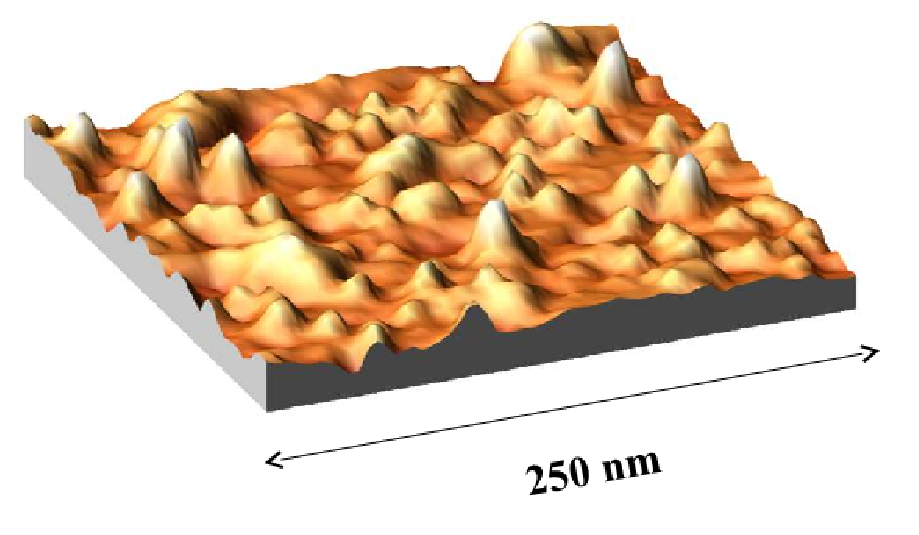
\includegraphics[width=8cm]{Pictures/AFMQD.eps}
	\end{center}}
	\end{figure}

	The effects of confinement on the carrier are generally described in the envelop function formalism. To define these envelop functions, we develop the carriers wave-functions on all the Bloch states:
	\begin{align}
		\Psi (\mathbf{r}) = \sum_{n,\mathbf{k}} c_{n,\mathbf{k}} \psi_{n,\mathbf{k}} = \sum_{n,\mathbf{k}} c_{n,\mathbf{k}} u _{n,\mathbf{k}} (\mathbf{r}) \exp (i\mathbf{k}.\mathbf{r})
	\end{align}
Since we are in a confined environment, we can consider only the states around $\mathbf{k} = 0$. Since we consider the band extrema, we neglect for this part the inter-band wave function mixing and use the effective-mass approximation. We can then limit the expansion of Bloch state to an expansion on the $u _{n,0} (\mathbf{r}) \exp (i\mathbf{k}.\mathbf{r})$, with $n = \Gamma_6$ for the conduction band and $n = \Gamma_8$ for the valence band. The sum on $\Gamma_8$ is equivalent to a sum on the $J_z = \{\pm \frac{3}{2}, \pm \frac{1}{2}\}$. We can then write:
	\begin{align}
		\Psi_c (\mathbf{r}) & \simeq \sum_{\mathbf{k}} u _{\Gamma_6,0} c_{\Gamma_6, \mathbf{k}} (\mathbf{r}) \exp (i\mathbf{k}.\mathbf{r}) = u _{\Gamma_6,0} F_e (\mathbf{r}) \label{eEnvFunc} \\		
		\Psi_v (\mathbf{r}) & \simeq \sum_{J_z = \{\pm \frac{3}{2}, \pm \frac{1}{2}\}, k} u _{\Gamma_8,J_z} c_{J_z,\mathbf{k}} (\mathbf{r}) \exp (i\mathbf{k}.\mathbf{r})  = \sum_{J_z = \{\pm \frac{3}{2}, \pm \frac{1}{2}\}} u _{\Gamma_8,J_z} F_{J_z} (\mathbf{r}) \label{hEnvFunc}
	\end{align}
with $F_e (\mathbf{r}) = \sum_{\mathbf{k}} c_{\mathbf{k}} \exp (i\mathbf{k}.\mathbf{r})$ the electron envelop function and $F_{J_z} (\mathbf{r}) = c_{J_z,\mathbf{k}} \exp (i\mathbf{k}.\mathbf{r})$, $J_z = \{\pm \frac{3}{2}, \pm \frac{1}{2}\}$ the hole envelop functions.

	The effective mass approximation allows us to replace the periodic crystal potential and the free-electron kinetic energy by the effective hamiltonians representing the band extrema. Considering the effective mass is the same in CdTe and ZnTe, we can now work with the simple picture of an effective mass carrier with the envelop function defined in Eqs.~\ref{eEnvFunc} and \ref{hEnvFunc}, trapped in a potential $V_e (\mathbf{r})$ for the conduction band or $V_h (\mathbf{r})$ for the valence band, created by the band offset between the two semiconductors. We write the Schrödinger equations for these particles:
	\begin{align}
		\left(\frac{\hbar^2}{2m_e}\Delta \right)F_e (\mathbf{r}) + V_e (\mathbf{r}) F_e (\mathbf{r}) &= E_eF_e (\mathbf{r}) \label{eSchroding} \\
		(\tilde{{\cal H}}_L + \tilde{{\cal H}}_{BP} + V_h (\mathbf{r})) 
			\begin{pmatrix}
				F_{+ \frac{3}{2}} (\mathbf{r}) \\
				F_{+ \frac{1}{2}} (\mathbf{r}) \\
				F_{- \frac{1}{2}} (\mathbf{r}) \\
				F_{- \frac{3}{2}} (\mathbf{r})
			\end{pmatrix}
			&= E_h
			\begin{pmatrix}
				F_{+ \frac{3}{2}} (\mathbf{r}) \\
				F_{+ \frac{1}{2}} (\mathbf{r}) \\
				F_{- \frac{1}{2}} (\mathbf{r}) \\
				F_{- \frac{3}{2}} (\mathbf{r})
			\end{pmatrix}
			\label{hSchroding}
	\end{align}
with $\tilde{{\cal H}}_L$ and $\tilde{{\cal H}}_{BP}$ the hole hamiltonians. In particular, we have to take the opposite of the electron hamiltonian defined in Eq.~\ref{LuttHamil}. In $\tilde{{\cal H}}_L$, the $k$-terms transform into a gradient of the envelop function with the form $i\nabla$. For simplicity, the $\tilde{}$ will be dropped in the next equations. The derivation of the effective mass approximation can be found in reference \cite{LuttElecMotion}.

	As pointed out in the end of Sec.~\ref{BPSec}, the gap between lh and hh is of about 300 meV, wide enough to neglect the lh contribution in first approximation. This is called the heavy hole approximation, decoupling the four differential equations defined in Eq.~\ref{hSchroding}. Only the ground states $|\pm \frac{3}{2}\rangle$ are considered, with the effective mass given by the diagonal term of ${\cal H}_{L}$, noted $m_{h, \parallel}$ in the plane and $m_{h, z}$ along the growth axis. The spin operator $J_x$, $J_y$ and $J_z$ can then be redefined in the heavy-hole space as $j_x$, $j_y$, $j_z$, written with the Pauli matrices like $\sigma_x$, $\sigma_y$ and $\sigma_z$.
	
	Even with those two approximations, the problem is not solvable analytically. However, it is possible for some chosen potentials. Let's consider a lens like quantum dot, with a radius in the $xy$ plane, noted $\rho$, much larger than its height $L_z$. We can therefore define two different harmonic oscillators: a 2D oscillator $V_{c,v} (\rho)$ in the plane, and a 1D oscillator $V_{c,v} (z)$ along the growth axis:
	\begin{align}
		V_{c,v} (\rho) = 4 \Delta E_{c,v} \frac{\rho ^2}{L_z^2} \\
		V_{c,v} (z) = 4 \Delta E_{c,v} \frac{z^2}{L_z^2}
	\end{align}
with $\Delta E_{c,v}$ the band offset between the two conduction (resp. valence) bands. The potential of the whole quantum dot will then be $V_{c,v} (\mathbf{r}) = V_{c,v} (\rho) + V_{c,v} (z)$. Separating the potential in those two parts means we are searching for solution of the form $F(z, \rho, \theta) = \chi (z) \phi_{n,m} (\rho, \theta)$, with $\theta$ the angle between the position vector and the $x$ axis.

	We write the characteristic spatial width $\sigma$ and characteristic frequency $\omega$ of the 2D harmonic oscillator felt by the hole:
	\begin{align}
		\Sigma_{\rho}^h &= \sqrt{\frac{\hbar}{m_{h, \parallel} \omega_{\rho}^{h}}} \\
		\omega_{\rho}^{h} &= \sqrt{\frac{8\Delta E_{v}}{m_{h, \parallel} L_{\rho}^2}}
	\end{align}
We can write the same equality along $z$ replacing $\rho$ by $z$ and $m_{h, \parallel}$ by $m_{h,z}$. The same can be done for electron, replacing the  $m_{h, \parallel}$ or $m_{h,z}$ by $m_e$ and $E_v$ by $E_c$.

	We can find in textbook such as ref.~\cite{MecQBasvant} the eigenstates of a harmonic oscillator from which we can deduce the eigenstates for the ground state (GS) and the first two degenerated excited states. The first excited state is found to have an angular momentum $l_z = \pm 1$, and is then noted $Exc, \pm 1$. The envelop functions and energy are then found to be:
	\begin{align}
			& F_{c,v}^{GS} (z, \rho, \theta) = \frac{1}{(\sqrt{\pi}\Sigma_z)^{\frac{1}{2}}} \exp \left(- \frac{z^2}{2 \Sigma_z^2}\right) \frac{1}{(\sqrt{\pi}\Sigma_{\rho})^{\frac{1}{2}}} \exp \left(- \frac{\rho^2}{2 \Sigma_{\rho}^2}\right) \label{GSWF} \\
			& E_{e,h}^{GS} = \hbar \frac{\omega_z^{e,h} + \omega_{\rho}^{e,h}}{2} \\
		\nonumber \\
			& F_{c,v}^{Exc, \pm 1} (z, \rho, \theta) = \frac{1}{(\sqrt{\pi}\Sigma_z)^{\frac{1}{2}}} \exp \left(- \frac{z^2}{2 \Sigma_z^2}\right) \frac{1}{(\sqrt{\pi}\Sigma_{\rho})^{\frac{1}{2}}} \exp \left(- \frac{\rho^2}{2 \Sigma_{\rho}^2}\right) \frac{\rho}{\sigma_{\rho}} \exp (\pm i\theta) \label{ExcWF} \\
			& E_{e,h}^{Exc, \pm 1} = \hbar \frac{\omega_z^{e,h} + 3 \omega_{\rho}^{e,h}}{2}
	\end{align}
We see that these energy levels are quantized in a way looking like an isolated atom. In reference to the atomic notation, the ground state, lower energy level, is noted $S$ and the two first degenerated level are noted $P$, even though atomic p-states usually are 3 fold degenerated.

	One remarkable feature of the envelop functions is that both GS and the two first excited states present the same envelop along the $z$ axis. The cause is directly the symmetry of the QD: since $L_z \ll L_{\rho}$, $\omega_z^{e,h} \gg \omega_{\rho}^{e,h}$, and since $E_{osc.\ harmo.} = (n+\frac{1}{2})\hbar \omega$, the next possible envelop function along the $z$ axis is at higher energy than the next one in the plane. This geometry is also responsible for the 2 fold degeneracy of the $P$-states.
	
	Both the GS and the excited states are once again degenerated due to the spin of the electron and the hole. The electron is in the conduction band with the $\Gamma_6$ symmetry: its spin along the $z$ axis is $\sigma_z = \pm \frac{1}{2}$ (noted $|\uparrow\rangle$ for $+\frac{1}{2}$ and $|\downarrow\rangle$ for $-\frac{1}{2}$). Since we are in the hh approximation, considering that the lh are far enough from the band edge to be negligible, the hole spin can only take the values $J_z = \pm \frac{3}{2}$ (noted $|\Uparrow\rangle$ for $+\frac{3}{2}$ and $|\Downarrow\rangle$ for $-\frac{3}{2}$). As pointed ahead, the hole is defined with the opposed characteristic of the missing electron. For instance, a hole $|\Downarrow\rangle$ corresponds to the absence of a valence electron $\Psi_v (\mathbf{r}) = u_{\Gamma_8, \frac{3}{2}} (\mathbf{r}) F_{\frac{3}{2}} (\mathbf{r})$.
	
	From the selection rules found in Sec.~\ref{k0Descr}, we can see that the only excitons able to recombine optically in the hh approximation are either formed by an electron of spin $\sigma_z = -\frac{1}{2}$ and a hole of angular momentum $J_z = +\frac{3}{2}$ (exciton of total angular momentum $X_z = +1$, recombining in $\sigma+$ polarization), or an electron of spin $\sigma_z = +\frac{1}{2}$ and a hole of angular momentum $J_z = -\frac{3}{2}$ (exciton of total angular momentum $X_z = -1$, recombining in $\sigma-$ polarization). Excitons of total angular moment $X_z = \pm2$ (electron spin $\sigma_z = \pm\frac{1}{2}$ with hole spin $J_z = \pm \frac{3}{2}$ exists, but cannot recombine optically.
	
	The addition of envelop functions in the carriers wave function adds another selection term:
	\begin{align}
		|\langle \Psi_v | \mathbf{p} | \Psi_c \rangle |^2 = |\langle F_v | F_c \rangle |^2|\langle u_{\Gamma_8, J_z} | \mathbf{p} | u_{\Gamma_6, \sigma_z} \rangle |^2
	\end{align}
The first term is the overlap of the envelop function, making sure the hole and the electron are of the right state. For instance, a transition between a $S$ state of the valence band and a $P$ state in the conduction band is then forbidden. The second term is the same as the one studied earlier, and from which we deduced the selection rules.

%	The second term, showing the interband matrix elements, depending only on the symmetry of the Bloch functions, will then draw the rule for the recombination. We use the notation define above to note the electron state in the conduction band. The valence band, formed by $p$ atomic states, three times degenerated, can be written from the $|X\rangle$, $|Y\rangle$ and $|Z\rangle$ electronic states as follows:
%	\begin{align}
%		|+1\rangle &= -\frac{|X\rangle + i|Y\rangle}{\sqrt{2}} \\
%		|0\rangle &= |Z\rangle \\
%		|-1\rangle &= \frac{|X\rangle - i|Y\rangle}{\sqrt{2}}
%	\end{align}
%We can now write the states of the conduction band by composing these electronic states to the spin states:
%	\begin{align}
%		|u_{\Gamma_8, +\frac{3}{2}}\rangle &= |+1\rangle|\uparrow\rangle \\
%		|u_{\Gamma_8, +\frac{1}{2}}\rangle &= \sqrt{\frac{2}{3}}|0\rangle|\uparrow\rangle + \sqrt{\frac{1}{3}}|+1\rangle|\downarrow\rangle \\
%		|u_{\Gamma_8, -\frac{1}{2}}\rangle &= \sqrt{\frac{2}{3}}|0\rangle|\downarrow\rangle + \sqrt{\frac{1}{3}}|-1\rangle|\uparrow\rangle \\
%		|u_{\Gamma_8, -\frac{3}{2}}\rangle &= |-1\rangle|\downarrow\rangle
%	\end{align}
%	Since we are working in the hh approximation, we neglect the contribution of the states $|u_{\Gamma_8, \pm \frac{1}{2}}\rangle$, calculating the interband matrix element only for $|u_{\Gamma_8, \pm \frac{3}{2}}\rangle$. Since $|\uparrow\rangle$ and $|\downarrow\rangle$ are orthogonal states, it is then clear that there is only two optically active transitions:
%	\begin{itemize}
%		\item between $|u_{\Gamma_6, \uparrow}\rangle$ and $|u_{\Gamma_8, +\frac{3}{2}}\rangle$ (hole $|\Downarrow\rangle$), coupled by $p_- = p_x - i p_y$, corresponding to $\sigma-$ photon absorption or emission.
%		\item between $|u_{\Gamma_6, \downarrow}\rangle$ and $|u_{\Gamma_8, -\frac{3}{2}}\rangle$ (hole $|\Uparrow\rangle$), coupled by $p_+ = p_x + i p_y$, corresponding to $\sigma+$ photon absorption or emission.
%	\end{itemize}
%	
%	We see thus that, for an exciton in the $S$ state of the QD, four configurations are possible. First, we have the bright states $|\uparrow \Downarrow \rangle$ for a $\sigma-$ absorption, with an angular momentum $X_z = \sigma_z + j_z = \frac{1}{2} - \frac{3}{2} = -1$; and $|\downarrow \Uparrow \rangle$, for a $\sigma+$ absorption, with an angular momentum $X_z = -\frac{1}{2} + \frac{3}{2} = +1$. Both of these states are optically active, meaning their transitions are permitted and they can recombine radiatively. Two other states, not able to recombine radiatively, can exists and are called dark states: $| \uparrow \Uparrow \rangle$, with an angular momentum $X_z = +2$, and $| \downarrow \Downarrow \rangle$, with an angular momentum $X_z = -2$.
	
	Approximating the QD potential as a harmonic potential usually overestimate the confinement, and thus the single-particle energy. But the wave-functions found in this chapter can still be used as trial wave-functions for variational calculations in other potential, in order to calculate the correct energy level.
	
%	We discussed in this chapter about the neutral exciton ($X$), formed by a single electron-hole pair. However, several types of exciton can be observed in a quantum dots. First to consider are the charged excitons. In this case, a supplementary charge is injected in the QD in addition to the exciton, forming a hole-hole-electron ($X^+$) or hole-electron-electron ($X^-$) complex. It also happen that two excitons with opposed spins are trapped in a dot. This complex is called biexciton, noted $X^2$, and relax to leave a single neutral exciton in the QD. Charged biexciton and other multi-exciton complex also exist but are not discussed in this thesis. Even if the physics of each of this systems is different, the selection rules devised in this chapter apply to all of them.

		\subsection{Electron-hole exchange in quantum dots\label{ehExch}}
		
%		Now that we established the basics of the interactions between carriers and magnetic atoms, we will do as we did in Sec.~\ref{e-hIntQD} and reduce the size of the studied semiconductor until reaching the quantum dot size and see how these interaction evolve with this reduction. Since both carriers and magnetic atom are now confine inside a small volume, the wave-functions have a bigger overlap and we can expect an increase of the exchange energies.

%		The simple picture of the interaction between the electron of the semiconductor we get in Sec.~\ref{ExchDMS} using the Hartree-Fock approximation is not enough to understand the emission spectrum we get from our quantum dots. We need to go more into details. For a few paragraphs, we go back considering a semiconductor without magnetic atoms. As shown in \cite{ExchSplitInteratomic}, we can treat the interaction between one electron in the conduction band and the $N-1$ electron of the valence band as an interaction between this electron and the corresponding hole, with an adding exchange interaction. We can then write the exchange hamiltonian in a Heisenberg form as:
%	\begin{align}
%	\label{ehExchHamil}
%		{\cal H}_{SC}^{exch} = I_{eh} \bm{\upsigma}.\mathbf{J}
%	\end{align}
%The matrix elements being:
%	\begin{align}
%		\langle e,h|{\cal H}_{SC}^{exch}| e', h' \rangle = \delta_{h,h'} \delta_{e, e'} (\epsilon_e - \epsilon_h) - K_{h'ee'h} + I_{eh'e'h}
%	\end{align}
%with $\epsilon_{e,h}$ the energy level of the electron and hole, $K_{h'ee'h}$ the direct Coulomb interaction and $I_{eh'e'h}$ the Coulomb exchange interaction.



%	We can then write the exchange hamiltonian in a Heisenberg form as:
%	\begin{align}
%	\label{ehExchHamil}
%		{\cal H}_{eh} = I_{eh} \bm{\upsigma}.\mathbf{J}
%	\end{align}
%with the matrix elements:
%	\begin{align}
%		\langle e,h|{\cal H}_{SC}^{exch}| e', h' \rangle = \delta_{h,h'} \delta_{e, e'} (\epsilon_e - \epsilon_h) - K_{h'ee'h} + I_{eh'e'h}
%	\end{align}
%with $\epsilon_{e,h}$ the energy level of the electron and hole, $K_{h'ee'h}$ the direct Coulomb interaction and $I_{eh'e'h}$ the exchange Coulomb interaction. As classically expected from an electric interaction between two opposite charges, the direct Coulomb interaction is attractive and therefore lower the overall energy of the system.

%	The Coulomb exhange interaction is written:
%	\begin{align}
%		I_{eh'e'h} = \frac{e^2}{4\pi \varepsilon} \int \mathrm{d}\mathbf{r}_1 \mathrm{d}\mathbf{r}_2 \frac{\psi_c^*(\mathbf{r}_1) \psi_{v'}^*(\mathbf{r}_2) \psi_{c'}(\mathbf{r}_2) \psi_v(\mathbf{r}_1)}{|\mathbf{r}_1 - \mathbf{r}_2|}
%	\end{align}
%with $\varepsilon$ the dielectric constant and $\psi_v$ the wave function of the missing exciton. One can see that it is different from zero only if the spin of the electron and the hole are opposite (meaning the spin of both electrons are the same). Since its value is positive for opposite electron and hole spins, this term will increase the energy of the bright states while the dark one remain unaffected. It results in a ferromagnetic effective hamiltonian lifting the degeneracy between between bright and dark states.






%PLAN :
% - Généralité sur l'interaction d'échange, son origine...
% - Dans le bulk -> interaction d'échange courte portée comme décrite: split noir et brillant.
% - BQ -> On passe en symmétrie $C_{2v}$. Confinement augmente l'inter d'échange courte portée. Mais la longue portée est aussi à prendre en compte et dépend de la forme de la boîte -> split les brillants (et participe donc au splitting noir brillant total également).
%     -> écriture du hamiltonien
% 				\begin{align}
%					{\cal H}_{eh}^{lr} &=
%					\begin{pmatrix}
%						\delta_0 & 0 & 0 & \delta_2 \\
%						0 & - \delta_0 & \frac{1}{2} \delta_1 \exp(-2i \phi_1) & 0 \\
%						0 & \frac{1}{2} \delta_1 \exp(-2i \phi_1) & -\delta_0 & 0 \\
%						\delta_2 & 0 & 0 & \delta_0
%					\end{pmatrix}
%				\end{align}
%	-> Détailler chacun des termes
% - Parler de l'émission comme fait dans paragraphe
% - Réduction de la symmétrie en $C_s$, citer article et matrice finale.

%	An electron in the conduction band of a semiconductor interacts with all the electrons of the valence band. Solving such a system would be impossible. However, as shown in \cite{ExchSplitInteratomic}, we can treat this interaction as an interaction between this given electron and the corresponding hole, with a direct term and an exchange one. As classically expected from an electric interaction between two opposite charges, the direct Coulomb interaction is attractive and therefore lower the overall energy of the system.

	%Bir et Pikus: l'interaction d'échange de coulomb de l'électron CB and les électrons VB peut être séparés en deux terme : un short range et un long range.
	
	Electrons are fermions, and thus are subjected to the Pauli exclusion principle. Being charged particles, they also interact with each other via the Coulomb interaction. Both of those have to be considered to write the interaction between the carriers in the semiconductor. It was shown by Wardzyński et al.~\cite{ExchSplitInteratomic} that the interaction between a conduction electron and all the electrons of the valence band can be written as an interaction between the considered electron and the corresponding hole. It can be separated into two terms: the direct Coulomb interaction, independent of the particles spins, and the exchange Coulomb interaction.
	
%Dire que le terme direct ne dépend pas du spind des particules ?
	
	In exciton, the direct Coulomb term is attractive, as classically expected from an electric interaction between two opposite charges. However, more complex systems can exist in a semiconductor: charged excitons X$^+$ (hole-hole-electron complex) and X$^-$ (hole-electron-electron complex), or biexciton X$^2$ (two excitons of opposite total angular momentum). Higher order multi-exciton or charged biexciton might also exists but they are not discussed in this thesis. In those multi-excitons, the total Coulomd interaction and the confinement make the system stable.

	Taking into account the symmetry of the crystal, Bir and Pikus demonstrated~\cite{BPExchInt} that the exchange hamiltonian between an electron of the conduction band and hole in the valence band can be decomposed in two different components:
	\begin{easylist}[enumerate]
		\ListProperties(Numbers=r, FinalMark={) })
		& For an electron and a hole in the same Brillouin zone, the short-range exchange interaction has to be considered. It can be written:
		\begin{align}
			\label{ShortRange}
			{\cal H}_{eh}^{sr} = I_{eh}^{sr} \bm{\upsigma}.\mathbf{j} + \sum_{i = x,y,z} b_i^{exch} \sigma_i j_i^3
		\end{align}
The first term lift the degeneracy between exciton of total angular moment $X=2$ and $X=1$. The second one takes into account the reduction of symmetry in a cubic lattice and gives the dark states a fine structure. This splitting is expected to be much smaller than the lift induced by $I_{eh}^{sr}$, but has never been observed experimentally in bulk semiconductor.
		& Carriers in different Brillouin-zone might be affected by the long-range exchange interaction. In bulk semiconductors, the long range term doesn't affect the bright exciton at $k = 0$. Since the radiative recombination we study occurs at $k=0$ in the studied semiconductors, the effects of the long range interaction are not visible via this probe.
	
	In a quantum dot, the confinement of the carrier leads to a better overlap of the wave function and thus greater short range exchange energies. Moreover, in an anisotropic potential, such as the one of Stransky-Krastanov dots (see Sec.~\ref{SK}), the long-range interaction mixes the bright excitons, splitting them in two levels. It is usually written as a $\delta_1$ term in the exchange hamiltonian.
	\end{easylist}
	%The splitting between the dark and bright excitons is thus also affected.

	Taking into account all these effects, we can the write the total exchange hamiltonian in the heavy hole exciton subspace ($X_z = |+2\rangle$, $|+1\rangle$, $|-1\rangle$, $|-2\rangle$):
	\begin{align}
	\label{Heh}
		{\cal H}_{eh} &= \frac{1}{2}
		\begin{pmatrix}
			\delta_0 & 0 & 0 & \delta_2 \\
			0 & - \delta_0 & \delta_1 \exp(-2i \phi_1) & 0 \\
			0 & \delta_1 \exp(2i \phi_1) & -\delta_0 & 0 \\
			\delta_2 & 0 & 0 & \delta_0
		\end{pmatrix}
	\end{align}
%with $\delta_1$ the splitting of the bright exciton induced by the exchange interaction.
with $\delta_0 = \frac{3}{2}I_{eh}$, representing the splitting between dark and bright exciton, $I_{eh} < 0$ being the electron-hole exchange constant; $\delta_1$ the splitting between the bright exciton states; and $\delta_2$ the fine structure of the dark exciton states. $\delta_0$ value is controlled both by long-range and short-range interaction, and is typically about 1 meV in CdTe/ZnTe. $\delta_1$ only appears in anisotropic QDs and is induced by the long-range interaction, varying between a few tens and a few hundreds of $\mu$eV. Finally, $\delta_2$ primarily arise from the short-range interaction.

%	In a quantum dot, the confinement of the carrier leads to a better overlap of the wave function and thus greater exchange energies. The exchange interaction has to be taken into account in order to fully understand the optical properties of such dots. Writing $\mathbf{j} = (j_z, j_+, j_-)$ and $\bm{\upsigma} = (\sigma_z, \sigma_+, \sigma_-)$, we can develop the exchange hamiltonian for a quantization axis along $z$:
%	\begin{align}
%	\label{HehC2v}
%		\begin{array}{rll}
%			{\cal H}_{e-h}^{exch, QD} &= \frac{2}{3}\delta_0 j_z \sigma_z &+ \dfrac{\delta_1}{2}\left(\exp (2i\varphi_1)j_+ \sigma_- - \exp (-2i\varphi_1)j_- \sigma_+ \right) \\
%										& &+ \dfrac{\delta_2}{2}\left(\exp (2i\varphi_1)j_+ \sigma_+ + \exp (-2i\varphi_1)j_- \sigma_- \right)
%		\end{array}
%	\end{align}
%with $\delta_0$ representing the splitting between dark and bright exciton, $\delta_1$ the splitting between the bright exciton states and $\delta_2$ the splitting between the dark exciton states. $\delta_0$ value is controlled both by long-range and short-range interaction, and is typically of about 1 meV in CdTe/ZnTe. $\delta_1$ only appear in anisotropic quantum dot and is induced by the long-range interaction, varying between a few tens and a few hundreds of $\mu$eV. Finally, $\delta_2$ primarily arise from the short-range interaction.
	
%	We note $\varphi_1$ the direction of the strain anisotropy in the QD.
	Calculating the eigenstate of the hamiltonian \ref{Heh}, we find that the long range interaction induce a linear polarization of the PL of the optically active states along $\varphi_1$ and $\varphi_1 + 90^{\circ}$ as follows:
	\begin{align}
		|\pi_{\varphi_1}\rangle = \frac{1}{\sqrt{2}}\left(\exp(-i\varphi_1)|+1\rangle + \exp(i\varphi_1)|-1\rangle\right) \\
		|\pi_{\varphi_1 + 90^{\circ}}\rangle = \frac{1}{\sqrt{2}}\left(\exp(-i\varphi_1)|+1\rangle - \exp(i\varphi_1)|-1\rangle\right)
	\end{align}
where $\varphi_1 = \dfrac{\pi}{4}$ corresponds to a polarization of the emission along the 110 axis.

	This model works well for quantum dots with an elongated lens shape ($C_{2v}$ symmetry), the shape taken for ideal QDs.  However, more realistic self-assembled QDs can have symmetries which can deviate quite substantially from the idealized shapes of circular or ellipsoidal lenses. For a $C_{s}$ symmetry (truncated ellipsoidal lens), additional terms coupling the dark and the bright excitons have to be included in the electron-hole exchange Hamiltonian. Following Ref. \cite{ZielinskiDarExc}, the general form of the electron-hole exchange Hamiltonian in the heavy-hole exciton basis for a low symmetry quantum dot (C$_s$) and a polarization along 110 is:
	\begin{align}
		\label{HehCs}
		\mathcal{H}_{eh} =\frac{1}{2} \left(
			\begin{array}{cccc}
			\delta_0                               &e^{-i\pi/4}\delta_{11}              &e^{i\pi/4}\delta_{12}        &\delta_2\\
			e^{i\pi/4}\delta_{11}                      &-\delta_0                       &e^{-i\pi/2}\delta_{1}       &-e^{i\pi/4}\delta_{12}\\
			e^{-i\pi/4}\delta_{12}                  &e^{i\pi/2}\delta_{1}           &-\delta_0                     &-e^{-i\pi/4}\delta_{11}\\
			\delta_2                 &-e^{-i\pi/4}\delta_{12}          &-e^{i\pi/4}\delta_{11}                     &\delta_0\\
			\end{array}
		\right)
\end{align}
		
		
		\subsection{Valence band mixing\label{VBM}}	
	
	We showed that the long range exchange interaction split the neutral exciton bright states in two linearly polarized lines, with a $90^{\circ}$ angle between them. However, this simple picture doesn't fit well with the data, such as presented in Fig.~\ref{XAlLinPol}. It is clear for the neutral species (X, X$^2$) that the angle between the polarization of the two lines is different from $90^{\circ}$. Moreover, the charged species (X$^+$, X$^-$) are found to present linear polarization dependencies. In those systems, the presence of two carriers (hole for X$^+$, electron for X$^-$) with opposite spin cancel out the electron-hole exchange interaction. Their linear polarization dependencies arise then from another phenomena.
	
	\begin{figure}[h!]
	\begin{center}
		\includegraphics[width=13cm]{Pictures/LinPol.png}
	\end{center}
	\caption{PL intensities of the bi-exciton (X$^2$), the charged excitons (X$^+$, X$^-$) and the neutral exciton (X) of a CdTe/ZnTe QD as the function of the angle of the linearly polarized detection. To simplify the reading, the intensities were also plotted on polar graph (bottom). Picture taken from Yoan L\'eger PhD thesis~\cite{YoanTh}.}
	\label{XAlLinPol}
	\end{figure}
	
	In order to understand the linear polarization dependency, we have include the light hole contribution. Looking at the general form of the Luttinger hamiltonian \ref{HLMat}, we see that it mixes heavy hole and light hole through its non-diagonal term $b_{Lutt}$ and $c_{Lutt}$. The Bir-Pikus hamiltonian \ref{BPHamil} presents the same symmetry and the same form as the Luttinger hamiltonian and thus also induces a coupling between the lh states and the hh states.
	
	In general, we can write the hamiltonian describing the influence of shape and strain on the valence structure in the ($|\dfrac{3}{2}, +\dfrac{3}{2}\rangle$, $|\dfrac{3}{2}, +\dfrac{1}{2}\rangle$, $|\dfrac{3}{2}, -\dfrac{1}{2}\rangle$, $|\dfrac{3}{2}, -\dfrac{3}{2}\rangle$) basis as:	
	\begin{align}
	\label{HVBM}
		{\cal H}_{VBM} =
		\begin{pmatrix}
			p+q & s & r & 0 \\
			s^* & p-q & 0 & r \\
			r^* & 0 & p-q & -s \\
			0 & r^* & -s^* & p+q
		\end{pmatrix}				
	\end{align}
%where $R = \delta_{xx,yy} - i \delta_{xy}$ describes the mixing induced by an anisotropy in the QD $xy$ plane, $Q = \delta_{xz} - i \delta_{yz}$ stands for an asymmetry in the plane containing the QD growth axis $z$, and $\Delta_{lh}$ is the splitting between lh and hh induced by the in-plane bi-axial strain and the confinement. The asymmetry described by $Q$ may come from the QD shape or the strain distribution. 
The induced hh/lh mixing is called Valence Band Mixing (VBM).

	Supposing a VBM only caused by strain anisotropy, its parameters can be written as function of the Bir-Pikus parameters and the crystal strain $\varepsilon_{ij}$ ($i,j = x$, $y$, $z$). The VBM parameters then writes~\cite{kpMethod}:
	%with $x$ the (100) axis of the crystal lattice and $z$ as defined above
	\begin{align}
		\label{VBMParam}
		p 	&= a_v Tr(\varepsilon) \\
		q	&= b \left(\varepsilon_{zz} - \frac{\varepsilon_{xx} + \varepsilon_{yy}}{2}\right) \\
		r	&= b \frac{\sqrt{3}}{2} (\varepsilon_{xx} - \varepsilon_{yy}) - id \varepsilon_{xy} \\
		s	&= d(\varepsilon_{xz} - i\varepsilon_{yz})
	\end{align}
The splitting between the hh states and the lh states can now be calculated in function of the Bir-Pikus parameters:
	\begin{align}
		\begin{array}{rl}
			\Delta_{lh} &= E_{\pm\frac{3}{2}} - E_{\pm\frac{1}{2}} = (p+q) - (p-q) \\
						&= 2b \left(\varepsilon_{zz} - \dfrac{\varepsilon_{xx} + \varepsilon_{yy}}{2}\right)
		\end{array}
	\end{align}
	
	If we now suppose a system with pure in-plane strain anisotropy ($r \neq 0$ and $s=0$), for an origin of the energy at the top of the valence band, i.e. the hh band, we can rewrite the VBM hamiltonian in the same basis as above as:
	\begin{align}
		{\cal H}_{VBM}^{in\ plane} =
		\begin{pmatrix}
			0 & 0 & \rho_s\exp(-2i\theta_s) & 0 \\
			0 & \Delta_{lh} & 0 & \rho_s\exp(-2i\theta_s) \\
			\rho_s\exp(2i\theta_s) & 0 & \Delta_{lh} & 0 \\
			0 & \rho_s\exp(2i\theta_s) & 0 & 0
		\end{pmatrix}
	\end{align}
with $\rho_s$ the strain coupling amplitude and $\theta_s$ the angle between axis of the strain induced anisotropy in the QD plane and the $x$ axis. One can notice that in the case of pure in-plane anisotropy, $|+\dfrac{3}{2}\rangle$ only mixes with $|-\dfrac{1}{2}\rangle$ and $|-\dfrac{3}{2}\rangle$ with $|+\dfrac{1}{2}\rangle$. An anisotropy along the $z$ axis, growth axis of the dots, is needed to mix $|\pm \dfrac{3}{2}\rangle$ with $|\pm \dfrac{1}{2}\rangle$. With this notation, in the limit of weak VBM, we can now rewrite the ground state of the holes as pseudo-spin in order to take the hh/lh mixing into account:
	\begin{align}
		|\tilde{\Uparrow}\rangle \propto |+\frac{3}{2}\rangle - \frac{\rho_s}{\Delta_{lh}}\exp(2i\theta_s)|-\frac{1}{2}\rangle \\
		|\tilde{\Downarrow}\rangle \propto |-\frac{3}{2}\rangle - \frac{\rho_s}{\Delta_{lh}}\exp(-2i\theta_s)|+\frac{1}{2}\rangle
	\end{align}
And we can define new angular momentum operator for these pseudo-spin:
	\begin{align}
		\tilde{J}_+ &= \frac{\rho_s}{\Delta_{lh}}
			\begin{pmatrix}
				0 & -2\sqrt{3}\exp(-2i\theta_s) \\
				0 & 0
			\end{pmatrix} \label{JtildeUP} \\
		\tilde{J}_- &= \frac{\rho_s}{\Delta_{lh}}
			\begin{pmatrix}
				0 & 0 \\
				-2\sqrt{3}\exp(2i\theta_s) & 0
			\end{pmatrix} \label{JtildeDOWN} \\
		\tilde{J}_z &=
			\begin{pmatrix}
				\dfrac{3}{2} & 0 \\
				0 & -\dfrac{3}{2}
			\end{pmatrix} \label{JtildeZ}
	\end{align}
$\tilde{J}_{\pm}$ are the ladder operators, flipping the hole spin, whereas $\tilde{J}_z$ return the spin value. This last operator shows these states are mainly hh. This pseudo spin description is usually enough to understand the effect of the VBM, and we will use it to study how it modifies the emission of the quantum dot.

%	This simple picture, however, don't represent accurately most of the experiment. In a lot of found dots, both $X$ and $X^2$ present two peaks with linear polarization dependency, as presented in Fig.~\ref{XAlLinPol}. This picture could be explained by the long-range exchange interaction, presented in Sec.~\ref{ExchDMS}. However, it predicts an angle between the two linearly polarized states of $90^\circ$, while the observed angle is far from this value. Moreover, in charged species, the electron (resp. hole) interact with two holes (resp. electrons) with opposite spins, leading to an absence of exchange interaction. Therefore, in the hh approximation, neither $X^+$ nor $X^-$ should present linear polarization dependency. However, such a dependency can be observed in actual dots.
%	
%	However, we saw in Sec.~\ref{e-hIntQD} that the hh approximation supposed neglecting lh contribution in the Luttinger hamiltonian, through the presence of biaxial strain lifting their degeneracy with hh. However, we can see in the Bir-Pikus hamiltonian (Eq.~\ref{BPHamil}) that introducing an anisotropic distribution of strain ($\varepsilon_{xx} \neq \varepsilon_{yy}$ or $\varepsilon_{ij} \neq 0$ with $i \neq j$) can mix hh states $J_z = \pm \frac{3}{2}$ and lh states $J_z = \mp \frac{1}{2}$. Such a mixing, called Valence Band Mixing (VBM) can also occur through the Luttinger hamltonian in an anisotropic dot ($L_x \neq L_y$), but it would be weaker than the one occurring through Bir-Pikus hamiltonian.
%	
%	Looking at the matrix form of the Luttinger hamiltonian in Eq.~\ref{HLMat}, we see that $\pm \frac{3}{2}$ could also be coupled to $\pm \frac{1}{2}$ through the $b$ term. However, we supposed that the wave function can be separated into a pure $z$ component and a pure $x - y$ one, meaning $\langle \chi_i (z) | k_z | \chi_j (z) \rangle = 0$ with $\chi_{(i,j)} (z)$ define in Eqs.~\ref{GSWF} and \ref{ExcWF}. This means $b$ doesn't couple envelop functions. A similar coupling parameter appear in the Bir-Pikus hamiltonian due to the shear strains $\varepsilon_{zx}$ and $\varepsilon_{zy}$. However, in most of the found dots, $\varepsilon_{zx}$ and $\varepsilon_{zy}$ is found to be negligible~\cite{YoanTh}.
%	
%	The envelop function mainly test the overlap and the energy state of the exciton. It doesn't affect light polarization. Therefore, in order to understand the effects of the VBM on the polarization of the dot emission, we can neglect them, only looking at the spin component. We also neglect the envelop function difference between hh and lh. We can then describe the coupling by redefining up and down hole spins as a superposition of $\pm \frac{3}{2}$ and $\mp \frac{1}{2}$. This lh part will be written through a phenomenological parameter $\eta \exp(2i \theta)$ with $\theta$ the direction of the strain:
%	\begin{align}
%		|\tilde{\Uparrow}\rangle \propto |+\frac{3}{2}\rangle - \eta \exp(2i \theta)|-\frac{1}{2}\rangle \\
%		|\tilde{\Downarrow}\rangle \propto |-\frac{3}{2}\rangle - \eta \exp(2i \theta)|+\frac{1}{2}\rangle
	%\end{align}
%with, in the hypothesis of a small strain-induced VBM:
%	\begin{align}
%		\eta \exp(2i \theta) = \frac{1}{\Delta_{lh}} (id\varepsilon_{xy} - b(\varepsilon_{xx} - \varepsilon_{yy}))
%	\end{align}
%with $\Delta_{lh}$ the lh-hh splitting given by the average in-plane bi-axial strain $b(\varepsilon_{xx} = \varepsilon_{yy} + 2\varepsilon_{zz})$. However, experimentally, we can only access $\eta = \frac{E}{\Delta_{lh}}$, with $E$ the anisotropy of strain.

	In order to do so, we begin to consider the emission of the negatively charged state X$^-$. Since, as explained earlier, the exchange interaction is zero in such systems, because of the opposite spin of the two electrons, it will allow us to focus on the effects of the VBM. We can ignore the envelop function, testing mainly the overlap of the carriers wave function and thus not affecting the polarization of the emission. We write the polarization of the detection $\mathbf{e} = \cos (\alpha) \mathbf{e_x} + \sin (\alpha) \mathbf{e_y}$. We then can find the oscillator strength of the transition:
	\begin{align}		
		\begin{array}{rl}
		\label{VBMPolar}
			\Omega (\alpha) &\propto |\langle \uparrow | \cos(\alpha)p_X + \sin(\alpha)p_Y | \uparrow \downarrow \tilde{\Uparrow} \rangle |^2 \\
							&= 1 + \dfrac{1}{3} \dfrac{\rho_s}{\Delta_{lh}}^2 + \dfrac{2}{\sqrt{3}} \dfrac{\rho_s}{\Delta_{lh}} \cos(2(\theta_s - \alpha))
		\end{array}
	\end{align}
with $\mathbf{p} = -i\hbar\bm{\nabla}$. Contrary to what is expected in the hh approximation, we see that the charged exciton can have a strong linear component, depending on the strength of the lh/hh mixing.

	In the QD presented in Fig.~\ref{XAlLinPol}, the linear polarization rate $\rho_l = \dfrac{2A}{1 + A^2} \approx 40\%$, with $A = \frac{\rho_s}{\sqrt{3}\Delta_{lh}}$ corresponding to a very strong lh-hh mixing, with $\frac{\rho_s}{\Delta_{lh}} \approx 0.75$. Experimentally, no correlation were found between the polarization axis of different QDs, neither with the crystallographic axis, nor between QDs close to each other. Such a behaviour can be explained considering the anisotropic relaxation of strains occurring during the growth of the QDs~\cite{VBMArticle}. This behaviour was also observed in III-V compounds at low QD density (near the 2D-3D transition), also attributed to the effect of strains~\cite{IIIVFastExcSpinRelax}. For the III-V system, this hypothesis is supported by AFM studies showing that, in such growth conditions, the dots are preferentially nucleating near structural defects~\cite{IIIVAFM}. In the case of II-VI materials, a strained induced hh/lh mixing is not surprising as the dislocation formation energy is lower in those material, as shown in Ref.~\cite{TinjodMBE}.

	For the charged states $X^+$ and $X^-$, only the VBM leads to this linear polarization. However, in $X$ and $X^2$, the VBM and the long range exchange interaction are in competition for the polarization of the emission. The strain tends to polarize linearly the PL along $\theta_s$ and $\theta_s + 90^{\circ}$, when the long range exchange interaction favour linear emission along $\varphi_1$ and $\varphi_1 + 90^{\circ}$. This explains that the angle between the two linearly polarized exciton lines is not equal to $90^{\circ}$. Moreover, the valence band mixing results in a fine structure splitting through the short range exchange interaction that can either enhance or decrease the fine structure splitting due to the long range exchange interaction. In order to illustrate our point, we consider only the isotropic part of the short range electron-hole exchange interaction described in Eq.~\ref{ShortRange}:
	\begin{align}
		{\cal H}_{eh}^{sr,iso} = I_{eh} \bm{\upsigma}.\mathbf{J}
	\end{align}
where $\frac{3}{2}I_{eh}$ corresponds to the energy splitting between bright and dark excitons due to the short range exchange interaction. The coupling between the bright states $|\downarrow \tilde{\Uparrow}\rangle$ and $|\uparrow \tilde{\Downarrow}\rangle$ through ${\cal H}_{eh}^{sr,iso}$ can be calculated using the pseudo-spin ladder operator defined in \ref{JtildeUP} and \ref{JtildeDOWN}:
	\begin{align}
		\langle \downarrow \tilde{\Uparrow} | {\cal H}_{eh}^{sr,iso} | \uparrow \tilde{\Downarrow}\rangle = \frac{1}{2\sqrt{3}} I_{eh} \frac{\rho_s}{\Delta_{lh}} \exp(-2i\theta_s)
	\end{align}
	
	Hence, the valence band mixing through the short range exchange interaction splits the bright states into two linearly polarized states along axis defined by the strain angle $\theta_s$. The competition between this effect and the long range exchange interaction results in an angle between the two linearly polarized states different from $90^{\circ}$, as observed in the emission of CdTe/ZnTe QDs~\cite{DELum} and in InAs/GaAs ones~\cite{PolarIIIV}. Dark states are also coupled to bright ones in second order, giving them a weak oscillator strenght, with a dipole along $z$. A more in depth investigation of these effects was done in Yoan L\'eger's PhD thesis~\cite{YoanTh}.

	
	\section{Exchange interaction between carrier and magnetic atom\label{Exch}}
	
		\subsection{Exchange interaction in diluted magnetic semiconductors\label{ExchDMS}}
		
		We are interested in thesis to introduce a low density of either Manganese or Chromium atoms in the crystal. A semiconductor doped this way is called Diluted Magnetic Semiconductor (DMS). The magnetic atoms interact with the semiconductor electrons via its localized electrons on its outside $d$ shell, via the exchange interaction. In this thesis, we are at the limit of what is considered a DMS: the density of magnetic atom (Mn and Cr) is about the same of the density of QDs. This way, statistically a few QDs contains a single magnetic atom per QD. This system can be used as a spin {\em qbit}. For Mn and Cr in CdTe, the outside $d$ shell is the $d$ orbital, so it will be the one considered in the following. From the interactions between these electrons and the one in the conduction band of the semiconductor, new properties will arise. We will write in this section the interactions between the different electrons of the semiconductor as a "Heisenberg" interaction:
		\begin{align}
			{\cal H}_{Heisenberg} = I \bm{\upsigma}.\mathbf{S}
		\end{align}
with $I$ the interaction constant, $\bm{\upsigma}$ the electron spin and $\mathbf{S}$ the spin of the magnetic atom.
	
	This interaction represents the Pauli exclusion principle through the interaction between two spins. All the interactions in this section will be of this form, although representing different physical processes, with only the interaction constant $I$ varying from one to another.
	
		\subsubsection*{Hamiltonian of a DMS}
	
	Both Cr and Mn are close in size to the Cd atoms they replace, so their insertion only induces a small perturbation in the crystal structure, meaning the semiconductor wave function will not be significantly altered by them. We can then, as usual, write the conduction electron wave function as $|\psi_{\mathbf{k}}\rangle|\sigma;\sigma_z\rangle \equiv |\psi_{\mathbf{k}};\sigma_z\rangle$, $|\psi_{\mathbf{k}}\rangle$ being the Bloch function of the electron. In a first time, we only consider electrons of the conduction band. On the other side, considering a magnetic atom at $\mathbf{r} = \mathbf{R_d}$, we write the spatial component of the wave function $\Phi_d (\mathbf{r} - \mathbf{R_d})$. Its total electronic spin, sum of the electron spins on its $d$ orbital, is noted $|S; S_z\rangle$. The whole wave function of the magnetic atom is then $|\Phi_d;S_Z\rangle$.
	
	Let's first consider the hamiltonian for single magnetic atom. Using Born-Oppenheimer approximation, separating the movement of the electrons from the one of the nuclei, we can write the hamiltonian for these electrons:
	\begin{align}
	\label{BOHamil}
		{\cal H}_{BO} = \sum_i \left(\frac{p_i^2}{2m_c} + V_c (\mathbf{r}_i) \right) + \frac{1}{2} \sum_{i,j} \frac{e^2}{4\pi \varepsilon_0 |\mathbf{r_i} - \mathbf{r_j}|}
	\end{align}
The first term is a single particle hamiltonian, taking into account the kinetic energy of the electron and the crystal potential $V_c (\mathbf{r}_i)$ felt by the electron at the position $\mathbf{r}_i$. This potential includes the impurities' potential, meaning it will be different at the impurities positions rather than elsewhere in the semiconductor. The final term represents the Coulomb interaction between the electrons.

	We can rewrite this hamiltonian using second quantification. We define the destruction (resp. creation) operator of a particle in the conduction band at the wave vector $\mathbf{k}$ and the spin $\sigma$ as $a_{\mathbf{k}, \sigma}$ (resp. $a_{\mathbf{k}, \sigma}^{\dagger}$). In the same way, we define the destruction (resp. creation) operator of the electronic level of an impurity as $a_{d, S}$ (resp. $a_{d, S}^{\dagger}$). Assuming the number of electrons on the $d$ orbital of the considered magnetic atom does not change, the hamiltonian \ref{BOHamil} then becomes:
	\begin{align}
			{\cal H}_{SQ} &= \sum_{\mathbf{k}, \sigma} E_{\mathbf{k}} a_{\mathbf{k}, \sigma}^{\dagger} a_{\mathbf{k}, \sigma} + \sum_{S} E_d a_{d, S}^{\dagger} a_{d, S} + \sum_{\mathbf{k}, \mathbf{k}'} U_{\mathbf{k}, \mathbf{k}'} a_{\mathbf{k}, \sigma}^{\dagger} a_{\mathbf{k}', \sigma} \nonumber \\
								&\qquad\qquad\quad+ \sum_{\mathbf{k}, \sigma, S} V_{kd} (a_{\mathbf{k}, \sigma}^{\dagger} a_{d, S} + a_{d, S}^{\dagger} a_{\mathbf{k}, \sigma}) + \frac{1}{2} \sum_{i,j,m,n} V_{i,j,m,n} a_i^{\dagger} a_j^{\dagger} a_n a_m \label{HamilSQ} \\
						&= {\cal H}_0 + {\cal H}_d + V_d + {\cal H}_{hyb} + {\cal H}_{Coulomb} \nonumber
	\end{align}
with $E_{\mathbf{k}}$, $E_d$, $U_{\mathbf{k}, \mathbf{k}'}$, $V_{kd}$ and $V_{i,j,m,n}$ the interactions constant. The constant electron number assumption is good enough for the picture we want to draw since most of the spin-driven interactions do not induce a change of this number.

	${\cal H}_0$ represents the energy of the unperturbed wave function of the semiconductor, with $E_k$ the energy of an electron with the wave vector $\mathbf{k}$.
	
	${\cal H}_d$ is the same as ${\cal H}_0$ but for an electron of the $d$ orbital of the considered magnetic impurity, with $E_d$ the energy of an electron on this orbital.
	
	$V_d$ represents the impurity potential, allowing the semiconductor electrons to scatter on it. However, in II-VI materials, both Mn and Cr are isoelectric impurities. Their modification to the host semiconductor potential is therefore negligible~\cite{DyakonovSpinPhysicsSC} and $|\psi_k\rangle$ can still be used as solutions for the electrons of the semiconductor.
	
	${\cal H}_{hyb}$, also called the Anderson hamiltonian, mixes the semiconductor states with the states of the impurities. It represents an exchange interaction between an electron of the semiconductor and one of the $d$ orbital of an impurity.

	${\cal H}_{Coulomb}$ is a two particles hamiltonian represents the direct and the exchange Coulomb interaction between the electrons of the semiconductor and of the impurity. $i$, $j$, $m$ and $n$ each represents a full wave function, both spatial and spin part, and can be either an electron of the semiconductor or of one of the impurities.
	
		\subsubsection*{The exchange interaction in DMS}

	We first focus on the action of ${\cal H}_{Coulomb}$. It can be separated in three different terms depending on the value of $i$, $j$, $m$ and $n$ as illustrated in Fig.~\ref{HybridEner}.
	
%	\begin{figure}[h!]
%	\begin{center}
%		\includegraphics[width=12cm]{Pictures/CrystalHamiltonians.png}
%	\end{center}
%	\caption{Different interactions derived from one particle hamiltonian. The wave-functions of the electron from the continuum and from the magnetic impurity are schematically drawn to show the hybridization arising from $H_{hyb}$. Impurity and lattice wave-functions are also drawn.}
%	\label{ExchInterIllust}
%	\end{figure}

	\begin{figure}[h!]
	\fcapside{\caption{Carrier interactions with no change of the number of electrons on the impurity, derived from the hamiltonian ${\cal H}_{Coulomb}$. Picture from Laurent Maingault PhD thesis~\cite{LaurentTh}.}\label{HybridEner}}
	{\begin{center}
		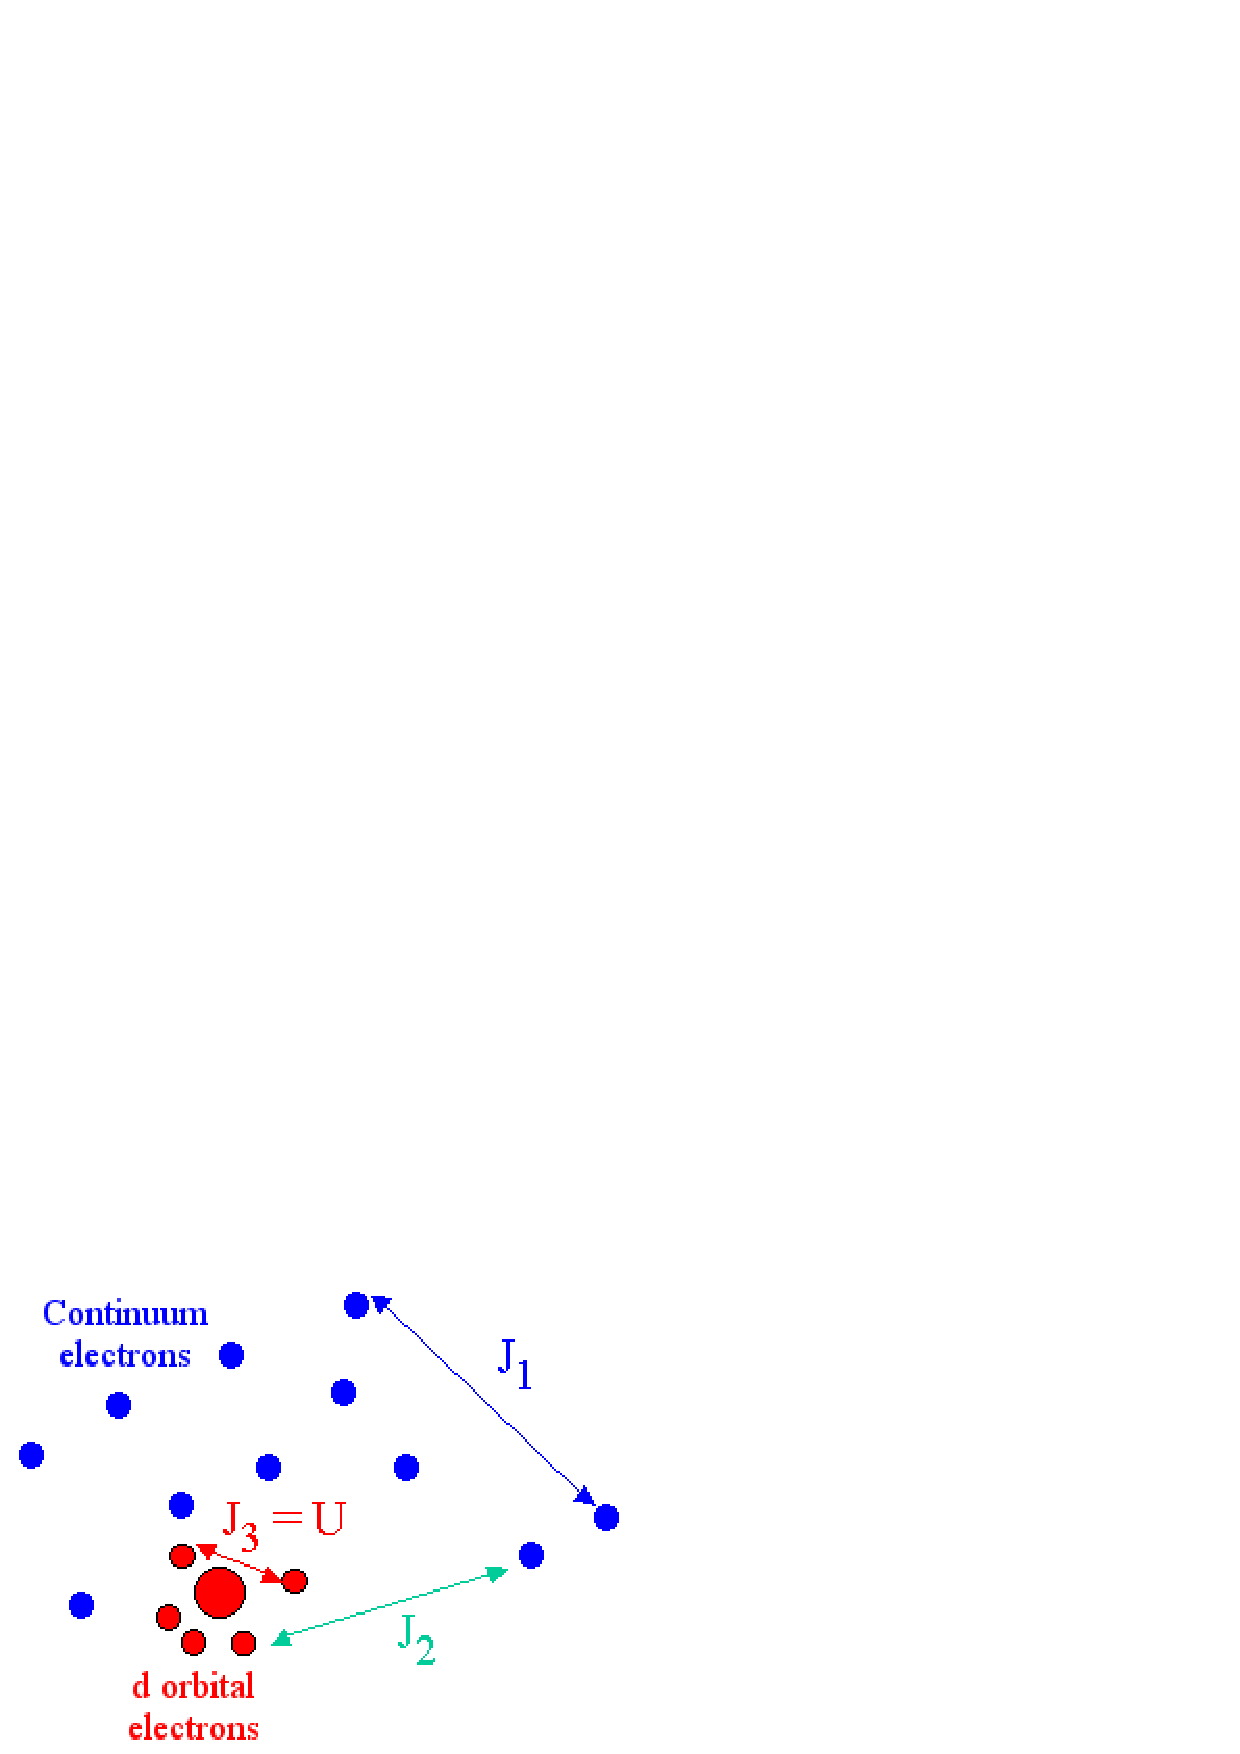
\includegraphics[width=6cm]{Pictures/ExchInt.png}
	\end{center}}
	\end{figure}

	Let's begin with the interaction noted $J_1$ on the diagram, two states belonging to the continuum of the semiconductors. This is the hamiltonian $H_{eh}$ introduced in Sec.~\ref{ehExch}.

%	Using Hartree-Fock approximation, considering all electron of the semiconductor except the one we look at as an effective electric field, we can include this term in the crystal potential, representing now both the potential of the ion lattice and the potential of the electrons. $V_{kd}$ will then use ${\cal H}_{HF}$ instead of ${\cal H}_1$:
%	\begin{align}
%	V_{kd} = \int \mathrm{d}\mathbf{r} \psi_k^* (\mathbf{r}) {\cal H}_{HF} \Phi_d (\mathbf{r} - \mathbf{R_d}) \label{Vkd}
%	\end{align}
%The interaction between the electron of the semiconductor will then be treated with more details in Sec.~\ref{ExchIntQD}.
	
	The next interaction we consider is the one of two electrons from a localized atom. It represents internal transitions of the atom, given by the Hund rule. It is written:
	\begin{align}
		{\cal H}_U = \sum_{d, S, S'} U a_{d, S}^{\dagger} a_{d, S'}^{\dagger} a_{d, S'} a_{d, S'}
	\end{align}
with $U = \int \mathrm{d}\mathbf{r} \mathrm{d}\mathbf{r'} \dfrac{e^2}{4\pi\varepsilon_0 |\mathbf{r} - \mathbf{r'}|} |\Phi_d (\mathbf{r})|^2 |\Phi_d (\mathbf{r'})|^2$ the Coulomb interaction between two electrons on the same orbital with different spins. Thus, it costs more energy to add an electron on the same orbital than on another. The Hund rule is verified, with electrons first filling all orbitals with parallel spin before adding an electron to an orbital with second one, with opposed spin.
	
	The third interaction is the one between an electron from the magnetic atom and an electron from the semiconductor. In the same way as with carriers of the bulk, it can be separated in two terms that will be developed in the next paragraphs: a direct Coulomb interaction between the two electrons, and an exchange interaction arising from the fermionic nature of electrons.
	
	The direct Coulomb interaction can be written:
	\begin{align}
		K &= + \sum_{\mathbf{k}, \sigma, \sigma'} K_{\mathbf{k}} a_{\mathbf{k}, \sigma}^{\dagger} a_{d, \sigma'}^{\dagger} a_{d, \sigma'} a_{\mathbf{k}, \sigma} \\
		\text{with} \nonumber \\
		K_k &= \int \mathrm{d} \mathbf{r} \mathrm{d} \mathbf{r}' |\psi_k (\mathbf{r})|^2 \frac{e^2}{4\pi \varepsilon_0 |\mathbf{r}' - \mathbf{r}|} |\Phi_d (\mathbf{r}')|^2 \nonumber
	\end{align}
It is clear that the spin $\sigma$ (resp. $\sigma'$) of the $\mathbf{k}$ electron (resp. $d$ electron) are not involved in this interaction: they are not changed by it. The wave vector $\mathbf{k}$ is also not affected by this interaction. The direct Coulomb interaction therefore only acts on the total energy of the system. The origin of the energy axis can be redefine to ignore it.

	The second term, the exchange interaction, written in second quantification, reads:
		\begin{align}
			J &= + \sum_{k, k', \sigma, \sigma'} I_{kk'}^{ex} a_{k', \sigma}^{\dagger} a_{d, \sigma'}^{\dagger} a_{k, \sigma'} a_{d, \sigma} = - \sum_{k, k', \sigma, \sigma'} I_{kk'}^{ex} a_{k', \sigma}^{\dagger} a_{k, \sigma'} a_{d, \sigma'}^{\dagger} a_{d, \sigma} \label{sdSQ} \\
			\text{with} \nonumber \\
			I_{kk'}^{ex} &= \int \mathrm{d} \mathbf{r} \mathrm{d} \mathbf{r}' \psi_{k'}^* (\mathbf{r}) \psi_{k}^* (\mathbf{r}') \frac{e^2}{4\pi \varepsilon_0 |\mathbf{r}' - \mathbf{r}|} \Phi_{d}^* (\mathbf{r}) \Phi_{d}^* (\mathbf{r}') \label{sdConst}
		\end{align}
As can be seen on Eq.~\ref{sdSQ}, this interaction exchange the spin $\sigma$ and $\sigma'$ of both electrons, as suggested by its name. Eq.~\ref{sdConst} shows that the spin interaction comes from a Coulomb interaction between two fermions.

	We define:
		\begin{align}
			\begin{array}{l}
				\sigma_{kk'}^z = a_{k, \sigma}^{\dagger} a_{k', \sigma} - a_{k, -\sigma}^{\dagger} a_{k', -\sigma} \\
				\sigma_{kk'}^+ = a_{k, \sigma}^{\dagger} a_{k', -\sigma} \\
				\sigma_{kk'}^- = a_{k, -\sigma}^{\dagger} a_{k', \sigma}
			\end{array}
		\end{align}
Considering now that this interaction does not change the number of electrons on the $d$ orbital of the considered magnetic atom, we can write the interaction as a Kondo hamiltonian~\cite{KacmanD0alphabetaIIVI}:
	\begin{align}
		\label{Exchsd}
		{\cal H}_{sd} = - \sum_{k, k'} I_{kk'}^{ex} \bm{\upsigma}_{k,k'}.\mathbf{S}
	\end{align}
Since $I_{k,k'}^{ex}$ is positive, the negative sign in front of the Kondo hamiltonian shows that the energy minimum is reached when the spins of both electrons are aligned, and is therefore ferromagnetic.
	
	We can now write the total hamiltonian \ref{HamilSQ}, breaking the hamiltonian ${\cal H}_{Coulomb}$ into its different part:
		\begin{align}
			{\cal H}_{SQ} &= {\cal H}_0 + {\cal H}_d + {\cal H}_{hyb} + {\cal H}_{eh} + {\cal H}_{U} + {\cal H}_{sd}
		\end{align}
		
		\subsubsection*{Orbital hybridization}

	We now have two hamiltonians to model the exchange interaction between the impurity and the semiconductor electrons: ${\cal H}_{sd}$ and ${\cal H}_{hyb}$. The first one was put in Heisenberg form in the previous section. This section will focus on the hybridization. The hybridization constant can be written as~\cite{AndersonHamil}:
	\begin{align}
	\label{Vkd}
		V_{kd} = \frac{1}{\sqrt{N}}\int \mathrm{d}\mathbf{r} \Phi_d^* (\mathbf{r} - \mathbf{R_d}) {\cal H}_{HF} (\mathbf{r}) \psi_k (\mathbf{r})
	\end{align}
with $N$ the number of primitive cell in the crystal and ${\cal H}_{HF} (\mathbf{r})$ the Hartree-Fock hamiltonian for a single electron.
	
	Schrieffer and Wolff rewrote the Anderson hamiltonian ${\cal H}_{hyb}$ in order to give a form closer to the Kondo hamiltonian~\cite{RelationAnderKondo}:
	\begin{align}
	\label{Ikk'}
			{\cal H}_{hyb} &= \sum_{k,k'} V_{kd} V_{k'd} \left(\dfrac{1}{E_k - (E_d + U)} + \dfrac{1}{E_{k'} - (E_d + U)}\right. \nonumber \\
			 				& \qquad \qquad \qquad \qquad \qquad \qquad \left. - \dfrac{1}{E_k - E_d} - \dfrac{1}{E_{k'} - E_d}\right)a_{k', \sigma}^{\dagger} a_{k, -\sigma} a_{d, S-2\sigma}^{\dagger} a_{d, S} \nonumber \\
			 				&= -  \sum_{k,k'} I_{kk'}^{hyb} a_{k', \sigma}^{\dagger} a_{k, -\sigma} a_{d, S-2\sigma}^{\dagger} a_{d, S}
	\end{align}
This form suppose that the magnetic atom $d$ levels are far from the band edge. This assumption works well for Mn. However, the Cr ground state is at the edge of the valence band. Therefore, knowing the sign of $E_k - E_d$ or $E_{k'} - E_d$ is more difficult~\cite{BlinowskyKinExchDMS}. In order to give an idea of the construction of the hybridization, we will focus on the Mn case. The case of the Cr will be discussed more in details in Sec.~\ref{CrCdTe}.

	\begin{figure}[h!]
	\fcapside{\caption{Schema of the band structure and virtual transitions between valence band and conduction band. Picture taken from Laurent Maingault's PhD thesis~\cite{LaurentTh}. $E_d$ is the ground energy of the $d$ electrons of the magnetic atom; $U$ is the energy needed for the magnetic atom to reach its first excited state; $E_v (k)$ is the valence band energy; $E_g (k)$ is the conduction band energy}\label{EnerTransit}}
	{\begin{center}
		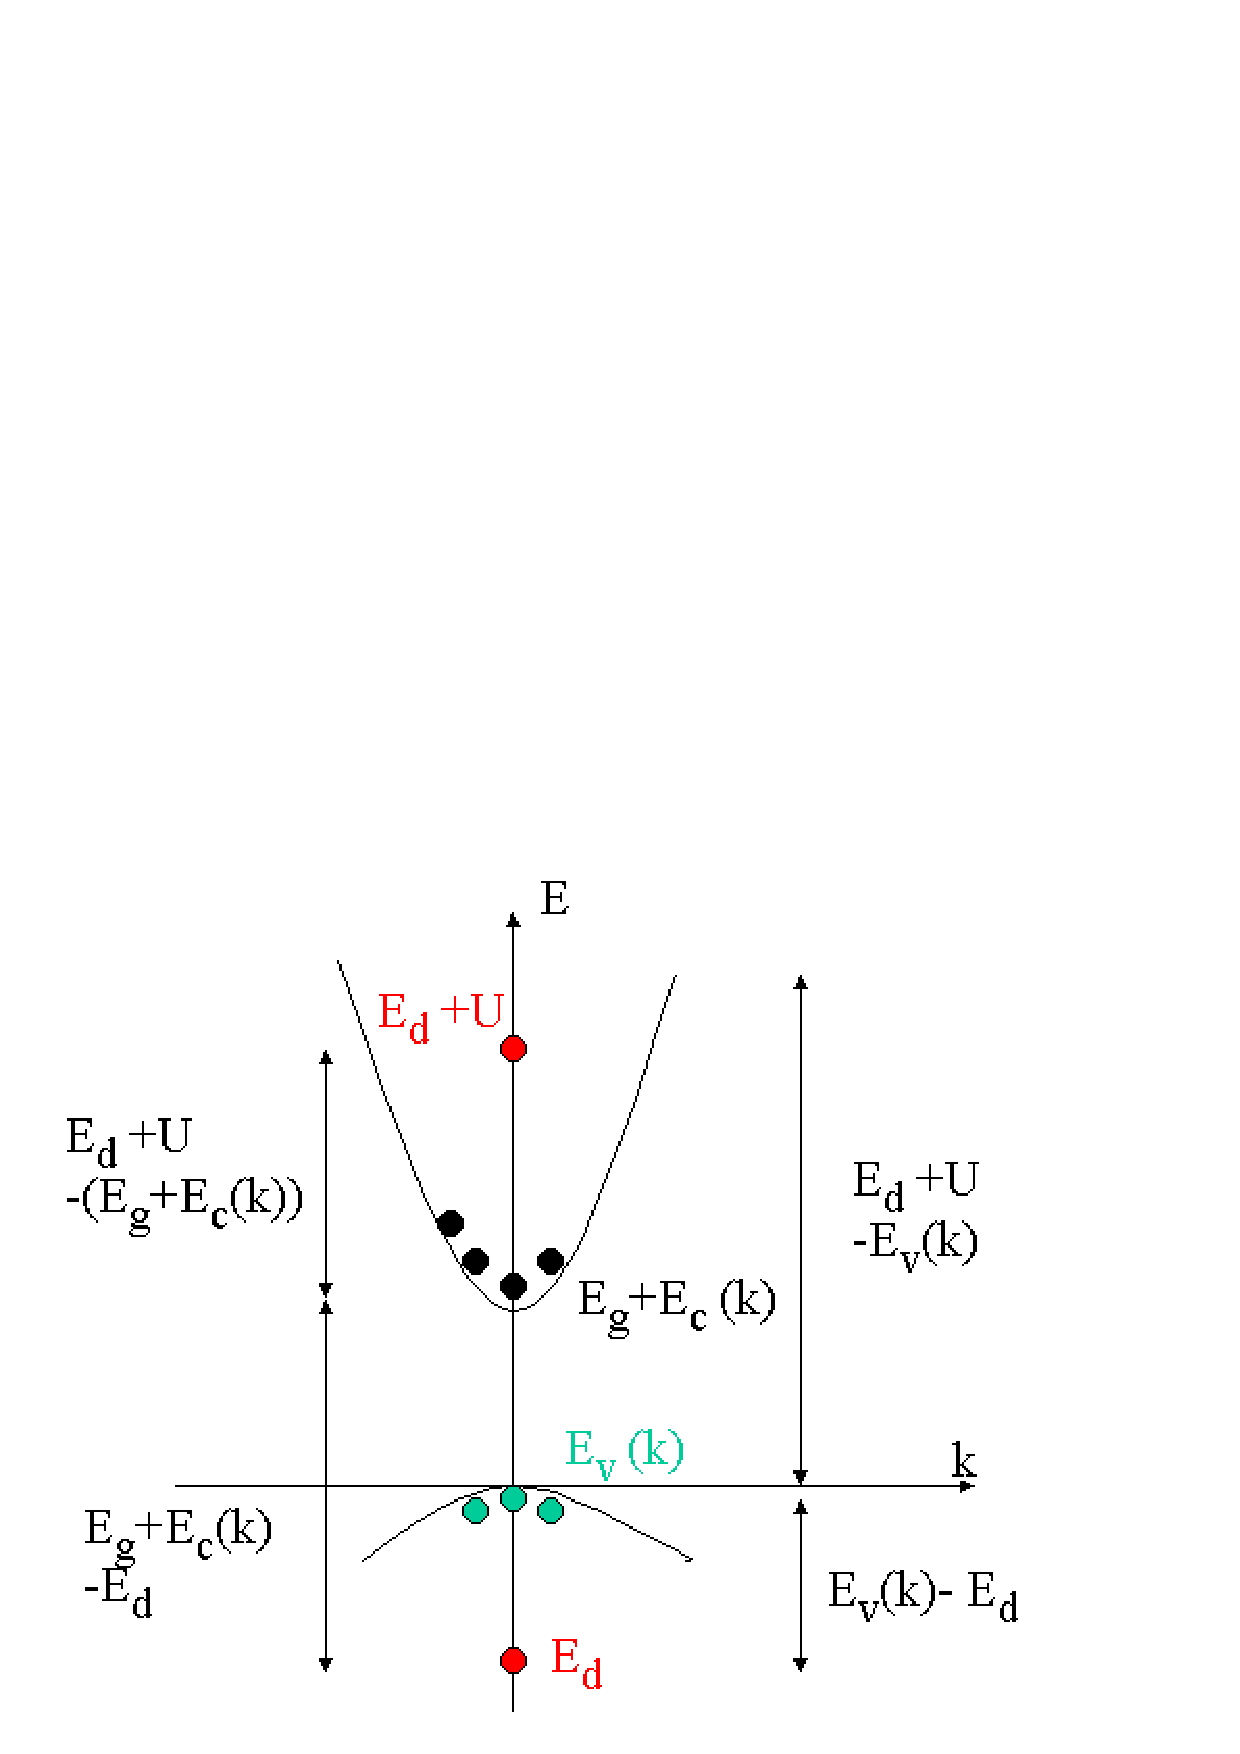
\includegraphics[width=7.6cm]{Pictures/EnergyLevels.png}
	\end{center}}
	\end{figure}
	
	The Fig.~\ref{EnerTransit} illustrates the different energies introduced in \ref{Ikk'}, presenting virtual transitions to the $d$ orbital of the magnetic atom. The two possible energies are $E_d$ for the low energy level, and $E_d + U$ for the high energy one, $U$ being the energy needed to add an electron to the orbital.

	Supposing the coupling occurs between two electrons with a close $k$ ($k \simeq k'$), we can rewrite $I_{kk'}^{hyb}$ as:
	\begin{align}
		\begin{array}{rl}
			I_{kk'}^{hyb} &= 2|V_{kd}|^2 \dfrac{U}{(E_k - E_d)(E_k - (E_d + U)} \\
						&= -2|V_{kd}|^2 \dfrac{U}{(E_k - E_d)(E_d + U - E_k)}
		\end{array}
	\end{align}
For a magnetic atom ground state is deep inside the valence band, as it is the case for the Mn atom, $U$ and $E_k - E_d$ are both positive, while $E_k - (E_d + U)$ is negative (see Fig.~\ref{EnerTransit}). Thus, $I_{kk'}^{hyb}$ is negative, and leads to an anti-ferromagnetic one.

\subsubsection*{Exchange constants in DMS}

	With this last transformation, it is now possible to use a Heisenberg type spin hamiltonian for all interactions instead of a hamiltonian mixing wave functions. The only difference between the interactions is in the exchange constant:  $I_{kk'}^{ex}$ for the exchange, and $I_{kk'}^{hyb}$ for the hybridization.

	Using the same hypothesis done on Sec.~\ref{BandStruct} of small $k$ value, and the value of $V_{kd}$ presented in Eq.~\ref{Vkd}, we can rewrite the exchange constant:
	\begin{align}
		I_{00, \{c,v\}}^{hyb} &= -2 \left(\frac{U}{(E_{\{c,v\}}(0) - E_d)(E_d + U - E_{\{c,v\}}(0))}\right) |V_{kd}|^2 \\
		I_{00, \{c,v\}}^{ex} &= \int \mathrm{d}\mathbf{r} \mathrm{d}\mathbf{r}' \psi_0^{*\{c,v\}} (\mathbf{r}) \Psi_d^* (\mathbf{r}) \frac{e^2}{4\pi \varepsilon_0 |\mathbf{r}' - \mathbf{r}|} \psi_0^{\{c,v\}} (\mathbf{r}) \Psi_d (\mathbf{r})
	\end{align}
It has been shown that these results can be used both in the conduction band and in the valence band of semiconductors~\cite{BhattacharjeeExchVB}.
	
	In the conduction band, the orbitals are $s$, and so we will write the interaction $I_{sd}$. However, since $s$ orbitals have a spherical symmetry, there is no hybridization contribution~\cite{BhattacharjeeExchVB}. The expression is then pretty easy:
	\begin{align}
		I_{sd} = I_{00, c}^{ex}
	\end{align}
As discussed earlier, this lead to a ferromagnetic coupling between the conduction band electrons and the magnetic atom.

	The valence band is formed by the $p$ orbital of the semiconductor matrix, as discussed in Sec.~\ref{BandStruct}. We then write $I_{pd}$ as the sum of the hybridization and the exchange contributions:
	\begin{align}
		I_{pd} =I_{00, v}^{hyb} +  I_{00, v}^{ex}
	\end{align}
The two interactions are in competition in the valence band, with the exchange interaction inducing a ferromagnetic coupling, and the hybridization inducing an anti-ferromagnetic one. The final sign of the interaction depends on the material, and is more discussed in Sec.~\ref{AtinCdTe}.

	The exchange interaction in the valence band can be rewritten for holes, using the total angular momentum $\mathbf{J}$ instead of the pure spin $\mathbf{S}$. However, since $J = 3/2$ and the exchange constant $I_{pd}$ has been defined for $S = 1/2$, the hole exchange hamiltonian have to be written using $I_{pd}/3$~\cite{BhattacharjeeExchVB}.
	
	The interaction between semiconductors carriers one magnetic atom in the Heisenberg notation:
%	\begin{align}
%	\label{HSingleAt}
%		{\cal H}_{SQ} = {\cal H}_0 + {\cal H}_{eh} + I_{sd} \bm{\upsigma}.\mathbf{S} + I_{pd} \mathbf{J}.\mathbf{S}
%	\end{align}	
	\begin{align}
	\label{HSingleAt}
	\renewcommand{\arraystretch}{1}
		\begin{array}{rlcccccc}
			{\cal H}_{SQ} &= {\cal H}_0 &+& {\cal H}_{eh} &-& \underbrace{I_{sd} \bm{\upsigma}.\mathbf{S}} &-& \underbrace{\dfrac{I_{pd}}{3} \mathbf{J}.\mathbf{S}} \\
						&= {\cal H}_0 &+& {\cal H}_{eh} &+& {\cal H}_{sd} &+& {\cal H}_{pd}
		\end{array}
	\end{align}
Since a DMS contain a small percentage of magnetic atoms, we can write the hamiltonian of the full semiconductor by summing up the interaction all the sites with magnetic atoms. We finally get:
%	\begin{align}
%	\label{HDMS}
%		\begin{array}{rlcccccc}
%			{\cal H}_{DMS} &= {\cal H}_0 &+& {\cal H}_{eh} &+& \underbrace{\sum_i I_{sd} (\mathbf{R}_i) \bm{\upsigma}.\mathbf{S}_i} &+& \underbrace{\sum_i I_{pd} (\mathbf{R}_i) \mathbf{J}.\mathbf{S}_i} \\
%							&= {\cal H}_0 &+& {\cal H}_{eh} &+& {\cal H}_{sd} &+& {\cal H}_{pd}
%		\end{array}
%	\end{align}
	\begin{align}
	\label{HDMS}
		{\cal H}_{DMS} &= {\cal H}_0 + {\cal H}_{eh} - \sum_i I_{sd} (\mathbf{R}_i) \bm{\upsigma}.\mathbf{S}_i - \sum_i I_{pd} (\mathbf{R}_i) \mathbf{J}.\mathbf{S}_i
	\end{align}

	This can be further simplified with two approximations. First, since a conduction electron sees a lot of different atomic sites, we can work with the mean value of the magnetic atoms spins, $\langle\mathbf{S} \rangle$, instead of their individual value $\mathbf{S}_i$. This is the mean field approximation, the magnetic atoms being seen as an effective magnetic field. And for the same reason, we can consider the electron interaction with each site of the crystal multiplied by the probability $x$ of being occupied by a magnetic atom, instead of summing only on the magnetic atoms positions. This is the virtual crystal approximation. We can then rewrite:
	\begin{align}
		\sum_i I_{sd} (\mathbf{R}_i) \bm{\upsigma}.\mathbf{S}_i = x \sum_{\mathbf{R}} I_{sd} (\mathbf{R}) \bm{\upsigma}.\langle \mathbf{S} \rangle
	\end{align}
Projecting along the quantization axis, we just replace $\bm{\upsigma}.\langle\mathbf{S} \rangle$ by $\sigma_z \langle S_z \rangle$. Since the atoms are seen as a magnetic field, they induce a degeneracy lift $\Delta E_c$ between the two spin values of conduction electron, $|\sigma_z = \pm \dfrac{1}{2} \rangle$:
	\begin{align}
		\Delta E_c = -N_0 x \alpha \sigma_z \langle S_z \rangle
	\end{align}
with $\alpha \propto I_{sd}^{00}$ the interaction constant between the impurity's and the conduction band's Bloch function at $\mathbf{k} = 0$, and $N_0$ the number of cell per volume.
	
	The same consideration can be done for valence band. It is written for heavy holes:
	\begin{align}
		\Delta E_v = -N_0 x \frac{\beta}{3} J_z \langle S_z \rangle
	\end{align}
with $\beta \propto I_{pd}^{00}$ the interaction constant between impurity's and the valence band's Bloch function at $\mathbf{k} = 0$.

		\subsubsection*{Interactions for $k \neq 0$}

	To be complete with the analysis, we should also take into account the confinement due to the quantum dot. This means the wave vector $\mathbf{k}$ of the carriers can be different from 0, leading to small perturbative effect on ${\cal H}_{sd}$ and ${\cal H}_{pd}$. This was done in details by Laurent Maingault in the Chap.~I.3 of his PhD thesis~\cite{LaurentTh}. It is shown that the hamiltonian changed as follow:
	\begin{align}
			{\cal H}_{sd} (\mathbf{R}) &= -\alpha \bm{\upsigma}.\mathbf{S} \left| F_c(\mathbf{R}) - A_2\left( \frac{\partial^2 F_c}{\partial z^2} (\mathbf{R}) + \frac{\partial^2 F_c}{\partial \rho^2}(\mathbf{R})\right) \right|^2 \nonumber \\
										&  \qquad \qquad \qquad - \beta \bm{\upsigma}.\mathbf{S} \left( (C_2 - B_2) \left| \frac{\partial^2 F_c}{\partial z^2} (\mathbf{R}) \right|^2 + C_2 \left| \frac{\partial^2 F_c}{\partial \rho^2} (\mathbf{R}) \right|^2 \right) \\
			{\cal H}_{pd} (\mathbf{R}) &= -\beta \mathbf{J}.\mathbf{S} |F_v(\mathbf{R}) - V_{kd} F_v''(\mathbf{R})|^2
	\end{align}
with $F_c(\mathbf{R})$ (resp. $F_v(\mathbf{R})$) the electron (resp. hole) envelop function, $F_v'' (\mathbf{R})$ the second derivative of the hole envelop function, and $A_2$, $B_2$, $C_2$ constant depending on the semiconductor lattice. For CdTe, $A_2 = 10.3$ \AA$^{-2}$, $B_2 = 0.781$ \AA$^{-2}$ and $C_2 = 19.8$ \AA$^{-2}$.

		\subsection{Insertion of Mn or Cr atom in a semiconductor lattice\label{AtinCdTe}}
		
		We will consider in the section the interaction between single magnetic atoms and the carrier trapped in quantum dots. Specifically, we will be interested in the interaction with a Manganese or a Chromium atom. This does not change significantly the picture we drew in the previous section. However, for the interaction between the semiconductor electrons and the magnetic atom $d$ electrons, we will have to also take into account the overlap between the magnetic atom and the carriers. For a magnetic atom A at the position $\mathbf{R}$, we define the exchange constant:
		\begin{align}
			I_{eA} &= - \alpha |F_c (\mathbf{R})|^2 \label{eAexch}\\
			I_{hA} &= - \frac{\beta}{3} |F_v (\mathbf{R})|^2 \label{hAexch}
		\end{align}
			
			\subsubsection*{Mn in CdTe\label{MnCdTe}}
		
		Mn has an electronic structure [Ar]3d$^5$4s$^2$. When inserted into CdTe, it substitutes a Cd atom ([Kr]4d$^{10}$5s$^2$). Both atoms are isolectronics and thus, as Cd, Mn bonds with the neighbouring Te atoms with its two $s$ electrons of its outer shell. In the semiconductor matrix, it is then Mn$^{2+}$ that has to be considered, with an electronic structure [Ar]3d$^5$. Since the $d$ orbital is five time degenerated (doubled when taking spin into account), it is half-full in the case of the Mn. Following Hund's rule, the spin of those electron are all aligned, leading to a total electronic spin $S_{Mn} = 5/2$ and a total orbital momentum $L = 0$.	
		
		Using the exchange constant defined in Eq.~\ref{eAexch} and \ref{hAexch}, we can rewrite the hamiltonian \ref{HSingleAt}:
		\begin{align}
		\label{HSingleMn}
			\begin{array}{rlccc}
				{\cal H}_{cMn} &=& {\cal H}_{eMn} &+& {\cal H}_{hMn} \\
								&=& I_{eMn} \bm{\upsigma}.\mathbf{S}_{Mn} &+& I_{hMn} \mathbf{J}.\mathbf{S}_{Mn}
			\end{array}
		\end{align}
We ignore ${\cal H}_0$ here since it only shift the energy of the system without affecting the spins exchange interactions. We can then write its spin operator as we did for the carriers in Sec.~\ref{BandStruct}:
	\begin{align}
		\begin{array}{rl}
			S_{Mn, x} &= \begin{pmatrix}
						0 & \frac{\sqrt{5}}{2} & 0 & 0 & 0 & 0 \\
						\frac{\sqrt{5}}{2} & 0 & \sqrt{2} & 0 & 0 & 0 \\
						0 & \sqrt{2} & 0 & \frac{3}{2} & 0 & 0 \\
						0 & 0 & \frac{3}{2} & 0 & \sqrt{2} & 0 \\
						0 & 0 & 0 & \sqrt{2} & 0 & \frac{\sqrt{5}}{2} \\
						0 & 0 & 0 & 0 & \frac{\sqrt{5}}{2} & 0
			  		\end{pmatrix} \\
			\\
			S_{Mn, y} &= \begin{pmatrix}
						0 & -\frac{i\sqrt{5}}{2} & 0 & 0 & 0 & 0 \\
						\frac{\sqrt{5}}{2} & 0 & -i\sqrt{2} & 0 & 0 & 0 \\
						0 & \sqrt{2} & 0 & -\frac{3i}{2} & 0 & 0 \\
						0 & 0 & \frac{3}{2} & 0 & -i\sqrt{2} & 0 \\
						0 & 0 & 0 & \sqrt{2} & 0 & -\frac{i\sqrt{5}}{2} \\
						0 & 0 & 0 & 0 & \frac{\sqrt{5}}{2} & 0
			  		\end{pmatrix} \\
			\\
			S_{Mn, z} &= \begin{pmatrix}
						\frac{5}{2} & 0 & 0 & 0 & 0 & 0 \\
						0 & \frac{3}{2} & 0 & 0 & 0 & 0 \\
						0 & 0 & \frac{1}{2} & 0 & 0 & 0 \\
						0 & 0 & 0 & -\frac{1}{2} & 0 & 0 \\
						0 & 0 & 0 & 0 & -\frac{3}{2} & 0 \\
						0 & 0 & 0 & 0 & 0 & -\frac{5}{2}
				   \end{pmatrix}
		\end{array}
	\end{align}

		In the conduction band, the electrons $s$ orbitals are orthogonal to the $d$ orbital of the Mn atom. No hybridization can then occur. Only the Coulomd interaction remain, leading to a standard ferromagnetic interaction between conduction band electrons and Mn electronic spin. Confirming this, $N_0 \alpha = 0.22 \pm 0.01$ eV was measured~\cite{GajMnD0alphabeta}.
		
		The deduction is a bit harder to work out in the valence band. Valence electrons $p$ orbitals are not orthogonal to Mn electrons $d$ orbital, meaning there is a competition between the standard ferromagnetic exchange interaction and the $pd$ hybridization. It turns out that the hybridization is stronger than Coulomb exchange interaction for Mn in II-VI semiconductor, leading to an anti-ferromagnetic interaction between holes and Mn electronic spin~\cite{KacmanD0alphabetaIIVI}. For Cd$_x$Mn$_{1-x}$Te, $N_0 \beta = -0.88 \pm 0.01$ eV was measured, confirming this anti-ferromagnetism of the interaction.~\cite{GajMnD0alphabeta}.

%		Both in conduction and valence band, Coulomd interaction induce a ferromagnetic coupling between the Mn and the electron. However, the $s$ orbital of the conduction band are orthogonal to the $d$ orbital of the electron localized on the Mn. Therefore, no hybridation could occur between those. In the valence band, the hybridization occur, creating a strong anti-ferromagnetic coupling between the Mn electrons and the band ones, compensating the ferromagnetic interaction coming from the Coulomb interaction.
%		
%		The coupling value were extracting from magneto-optical experiment for Cd$_{1-x}$ Mn$_x$ Te and were found to be $N_0 \alpha = 0.2$ eV and $N_0 \beta = -0.88$ eV. This confirm the deduction we did on the previous paragraph, and show that the valence band interaction, represented by $N_0 \beta$, is stronger than the coupling with conduction electrons. It will be the main driver of the spin interactions in the system.
%		
%		We now can rewrite the hamiltonian \ref{HSingleMn} to make the sign of these interactions appears explicitly:
%	\begin{align}
%		{\cal H}_{Mn} &= - I_{eMn} \bm{\upsigma}.\mathbf{S} + I_{hMn} J_z.S_z - \frac{2}{3} I_{eh} J_s.\sigma_z
%	\end{align}
%The vector product between $\bm{\upsigma}$ and $\mathbf{S}$ is kept because the interaction is homogeneous, unlike interaction between Mn and hole spins.
	
			\subsubsection*{Cr in CdTe\label{CrCdTe}}
		Cr as an electronic structure [Ar]3d$^4$4s$^2$. Cr is also iso-electronic with the Cd and thus is introduced in the lattice in substitution to this atom, bonding with its two $s$ electrons and thus being inserted as [Ar]3d$^4$. Following Hunds rule for the Cr $d$ orbital, with find that Cr in CdTe has a total electronic spin $S_{Cr} = 2$ and a total orbital momentum $L=2$.
		
		As done with the Mn, we can rewrite the hamiltonian~\ref{HSingleAt} using the exchange interaction defined in the introduction of this section:
		\begin{align}
		\label{HCrDMS}
			\begin{array}{rlccc}
				{\cal H}_{cCr} &=& {\cal H}_{eCr} &+& {\cal H}_{hCr} \\
									&=& I_{eCr} \bm{\upsigma}.\mathbf{S}_{Cr} &+& I_{hCr} \mathbf{J}.\mathbf{S}_{Cr}
			\end{array}						
		\end{align}
Once again, we ignore ${\cal H}_0$ since it did not affect the spins exchange interaction. We can also write the Cr spin operators as follows:
	\begin{align}
		\begin{array}{rl}
			S_{Cr, x} =& \begin{pmatrix}
					0 & 1 & 0 & 0 & 0 \\
					1 & 0 & \sqrt{\frac{3}{2}} & 0 & 0 \\
					0 & \sqrt{\frac{3}{2}} & 0 & \sqrt{\frac{3}{2}} & 0 \\
					0 & 0 & \sqrt{\frac{3}{2}} & 0 & 1 \\
					0 & 0 & 0 & 1 & 0
				   \end{pmatrix} \\
			\\
			S_{Cr, y} = i&
				   \begin{pmatrix}
					0 & -1 & 0 & 0 & 0 \\
					1 & 0 & -\sqrt{\frac{3}{2}} & 0 & 0 \\
					0 & \sqrt{\frac{3}{2}} & 0 & -\sqrt{\frac{3}{2}} & 0 \\
					0 & 0 & \sqrt{\frac{3}{2}} & 0 & -1 \\
					0 & 0 & 0 & 1 & 0
				   \end{pmatrix} \\
			\\
			S_{Cr, z} =& \begin{pmatrix}
					2 & 0 & 0 & 0 & 0 \\
					0 & 1 & 0 & 0 & 0 \\
					0 & 0 & 0 & 0 & 0 \\
					0 & 0 & 0 & -1 & 0 \\
					0 & 0 & 0 & 0 & -2
				   \end{pmatrix}
		\end{array}
	\end{align}
		
		In the conduction band, the situation is the same as with Mn: the conduction electrons $s$ orbital are orthogonal to the Chromium $d$ orbital, and the hybridization is then zero. Only the Coulomb interaction remains and induces a ferromagnetic coupling between the electrons of the band and the Cr electronic spin. $N_0 \alpha$ was never measured in Cd$_x$Cr$_{1-x}$Te, but most magnetic atoms in II-VI semiconductor presents a value between $0.2$ eV and $0.3$ eV. It is then generally assumed that, in II-VI semiconductor, $N_0 \alpha \approx 0.2$ eV~\cite{MacspdexchCr}. We also chose to use this value.
		
		%Once again, valence band is a bit 
		In the valence band, the picture for Cr in CdTe is a lot more complicated and still open to discussions. The position of the $d$ ground state energy relative to the semiconductor valence band is critical and can make the kinetic exchange interaction change sign (see Fig.~\ref{EnerTransit} and Eq.~\ref{Ikk'} for a $d$ level energy $E_d$ in the gap). Cr 3$d$ level is almost at the same energy as the top of CdTe valence band, making it hard to decide whether it is in the gap or not.
		%It was however predicted that the sign of the interaction could change between hh and lh~\cite{WojtowiczXNewDMS}.
		
		$N_0\beta$ was never directly measured in Cd$_x$Cr$_{1-x}$Te and is challenging to find theoritically for the reason stated in the previous paragraph~\cite{BlinowskyKinExchDMS}. Wojtowicz et al. measured the Zeeman spin splitting of 1$S$ excitons in a quantum well. The results were coherent with an interaction of opposite signs for lh and hh~\cite{WojtowiczXNewDMS}. The evolution suggest a ferromagnetic interaction for hh and antiferromagnetic for lh. $N_0 \beta$ was found positive (ferromagnetic) in Cd$_x$Cr$_{1-x}$S~\cite{MacCdCrSD0beta} and in all the studied Zn based II-VI semiconductors, assuming $N_0 \alpha = 0.2$ eV~\cite{KacmanD0alphabetaIIVI}. Especially, in ZnTe, for $N_0 \alpha = 0.2$, a large ferromagnetic $N_0 \beta = +3.6 \pm 1.2$ eV was found~\cite{MacspdexchCr}. Since there is almost no valence band offset between ZnTe and CdTe and that the transition metal impurity levels does not significantly changes between compounds with common anions~\cite{KossutHandbook}, it could be reasonable to assume that $N_0 \beta$ in bulk CdTe is positive, giving a ferromagnetic hole-Cr interaction. However, any parameter that can change the position of the relative energies of the top of the valence band and of the $d$ orbitals, such as strain or the confinement, can affect the sign of this interaction.


	\section{Fine and hyperfine structure of a magnetic atom in II-VI semiconductors}

		\subsection{Mn atom in II-VI semiconductors~\label{MnSemiCon}}
		
%Début à refaire
%Plan:
%	- Mn libre = [Ar]3d$^5$4s$^2$ remplace Cd ([Kr]4d$^{10}$5s$^2$) dans la matrice. Deux électron s utilisés pour la liaisons -> devient Mn$^{2+}$, 3d$^5$. Couche externe d à moitié pleine: S = 5/2, L = 0. Pas d'effet des contraintes sur l'état fondamental.
%	- Développer les états excités.
%	- Splitting des états excités par le CF.
%	- Application des contraintes -> toujours pas d'effet sur l'état fondamental.
% 	- Application du Spin-Orbite -> splitting du à $D_0S_z^2$

%		{\huge REWRITE HERE}
		
	We saw that the Mn $d$ orbital is the outside orbital for Mn in CdTe and is half-filled, with 5 electrons on it. Following Pauli exclusion principle, this gives the Mn atom in a CdTe lattice an angular momentum $L = 0$.

%		Mn is incorporated in II-VI semiconductors as Mn$^{2+}$. This ion is really weakly coupled to the strain state at its position. In first approximation, we can then consider it as an isolated ion occupying a cation site in the lattice. We will first study the free ion and then see the effect of the lattice on the different states.
%		
%		The Mn$^{2+}$ electronic structure [Ar]$3d^5$. 
		
		We get from Hund's rule that adding an electron to an half-filled orbital has a high energy cost. The lowest energy excited states are therefore the flipping of an electron. For a free atom, it leads to a first excited state with an angular moment $L = 4$. Following the spectroscopic notation of these states $^{(2S+1)}L$, the ground state is noted $^6$S ($L=0$, $S = \frac{5}{2}$) and the first excited state is $^4$G ($L = 4$, $S = \frac{3}{2}$). Higher energy excited states also exist, but have no influence in our study. We can safely neglect them.
		
	\begin{figure}[h!]
	\begin{center}
		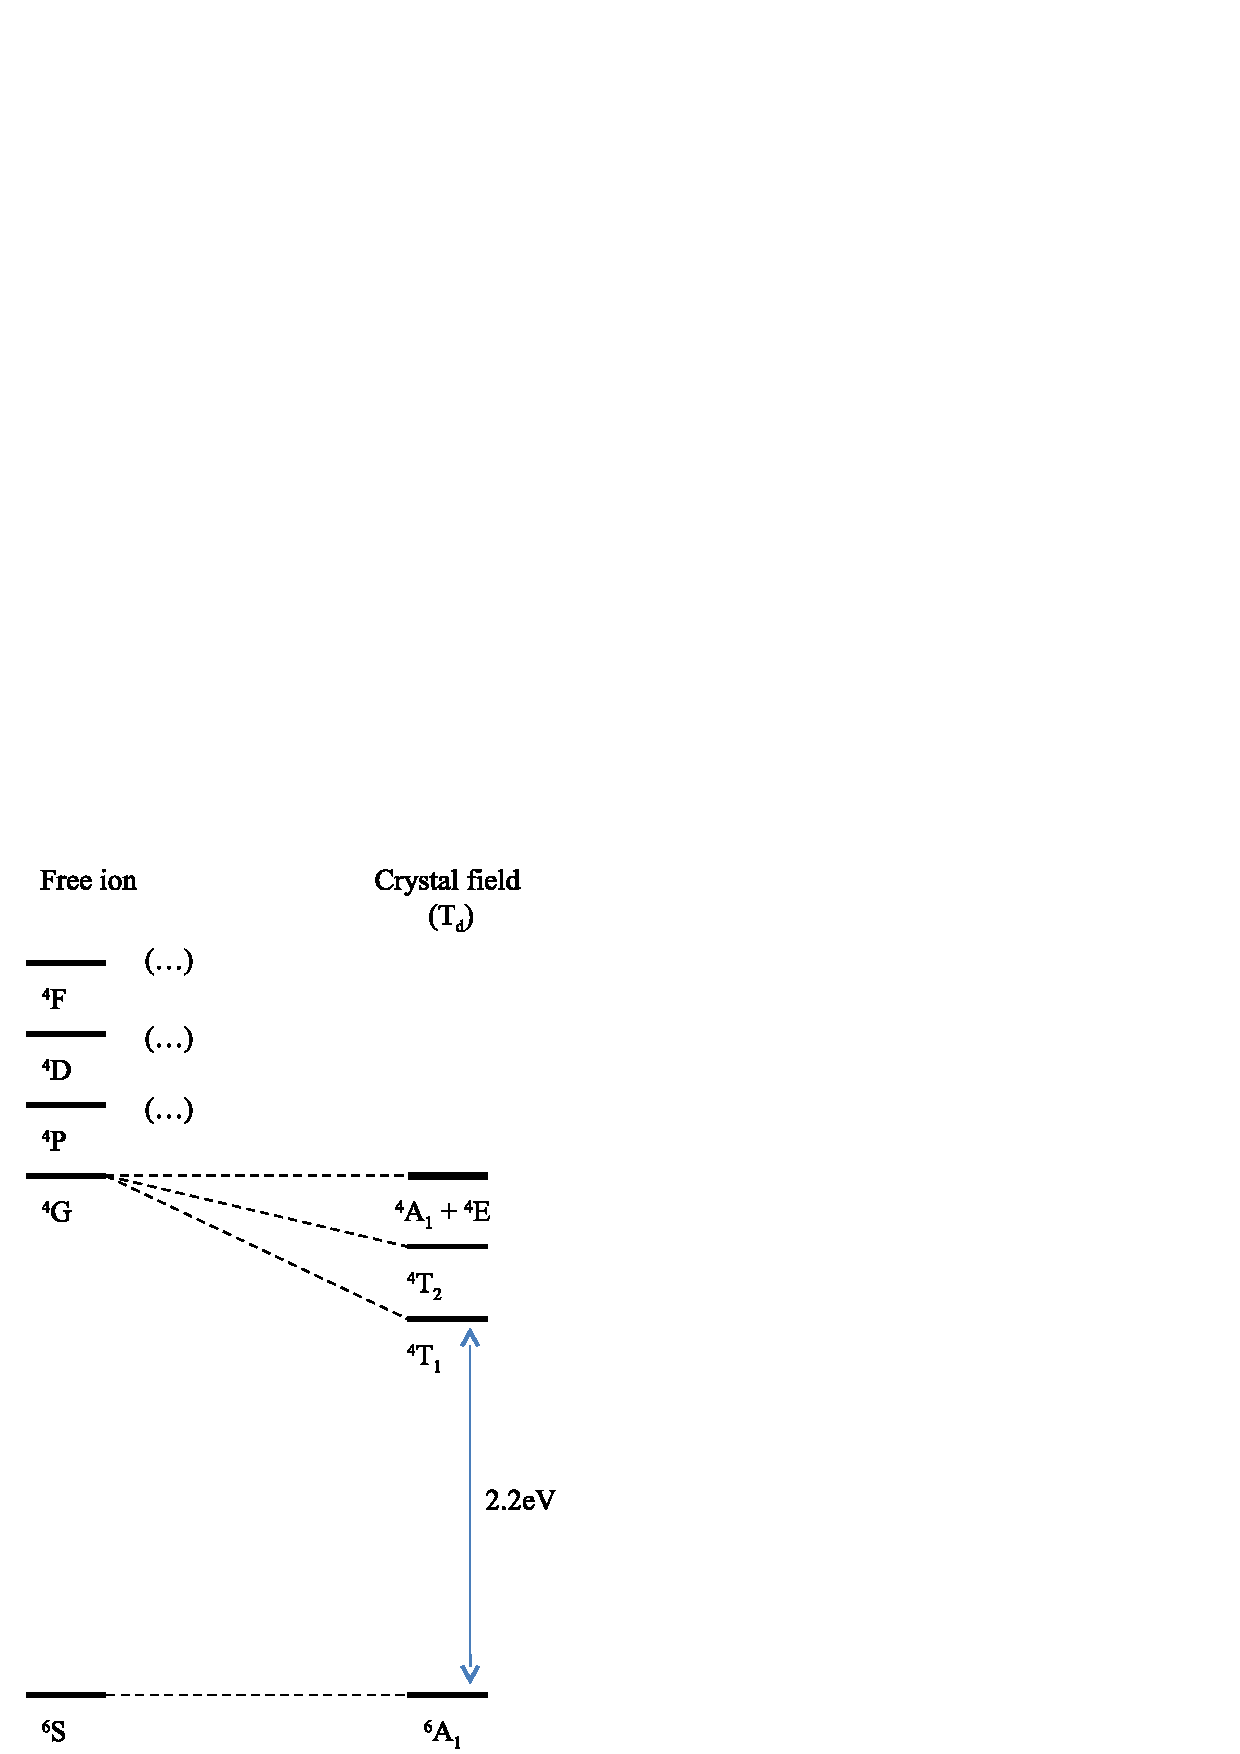
\includegraphics[width=10cm]{Pictures/MnCrystal.png}
	\end{center}
	\caption{Schematic diagram of the effect of the crystal field, biaxial strain and spin-orbit coupling on the Mn$^{2+}$ 3$d^5$ ground state ($^6$S). Effect of the crystal field on the first excited state ($^4$G) are also presented.}
	\label{MnCrystal}
	\end{figure}
		
		When inserted in the semiconductor matrix of $T_d$ symmetry, the interaction with the crystal field will lift the degeneracies of the free atom level. Those new levels are written with the appropriate group theoritical transformation properties. The $^6$S ground state is symmetrical and non-degenerated, except for spin. Thus, it is not affected by the crystal field and is noted $^6$A$_1$. On the other hand, $^4$G, the first excited state, has an orbital degeneracy and therefore is affected by the crystal field. It split into four different states: $^4$T$_1$, three-fold degenerated ; $^4$T$_2$, three-fold degenerated ; $^4$E, two-fold degenerated ; and $^4$A$_1$, not degenerated. It has been shown by calculations~\cite{TanabeGroupThMn,SolidStatesPhysics,ThTransMetalIon} that the effect of the crystal field is to pull the two $^4$T levels closer to the ground state, while $^4$E and $^4$A$_1$ are weakly affected by the crystal field.

	For a free atom, the transition between the ground state with $S=\frac{5}{2}$ and any of the excited states, with $S = \frac{3}{2}$ is forbidden by the $\Delta S = 0$ rule and the parity selection ones. However, in a II-VI lattice, the spin-orbit interaction and the absence of inversion symmetry relax those rules. The transitions between $^6$A$_1$ and the different states coming from the $^4$G splitting are allowed. $^6$A$_1 \rightarrow ^4$T$_1$ is the lowest energy of those transitions and therefore the most significant. It corresponds to approximately 2.2 eV. This transition can kill the luminescence of a semiconductor: the electron-hole recombination excite a $d$ electron instead of emitting a photon. However, this transition is unlikely to happen. For high concentration of Mn, it will significantly reduces the photoluminescence of the sample. However, we work at a really low concentration of Mn atoms in order to have QD with only one of them. This phenomena shouldn't then have a noticeable effect on our samples.
	
%	We saw in Sec.~\ref{BandStruct} that CdTe band gap was 1.6 eV at 5K, far from the Mn internal transition energy. The confinement, however, will increase the energy of the carriers in the quantum dot, getting them closer to the internal transition. To keep a strong enough luminescence, we then have to be wary of the size of our studied dots in order to stay far enough from these Mn transitions.

	$^6$A state of the Mn$^{2+}$ has no orbital degeneracy and thus is not affected by the T$_d$ crystal field nor by the reduction of its symmetry by the biaxial strain.  However, the spin degeneracy is lifted by a combination of spin-orbit interaction and reduced symmetry of the crystal field. In the presence of biaxial strain, this will results in a splitting the spin level according to $D_0S_z^2$~\cite{D0Sz}, with $D_0$ the magnetic anisotropy and $S_z$ the Mn spin quantized along the $z$ axis. Due to the null Mn orbital momentum ($L = 0$), the magnetic anisotropy is however weak and the spin splitting is only of a few tens of $\mu$eV, depending on the strains.
	
	\begin{figure}[h!]
	\begin{center}
		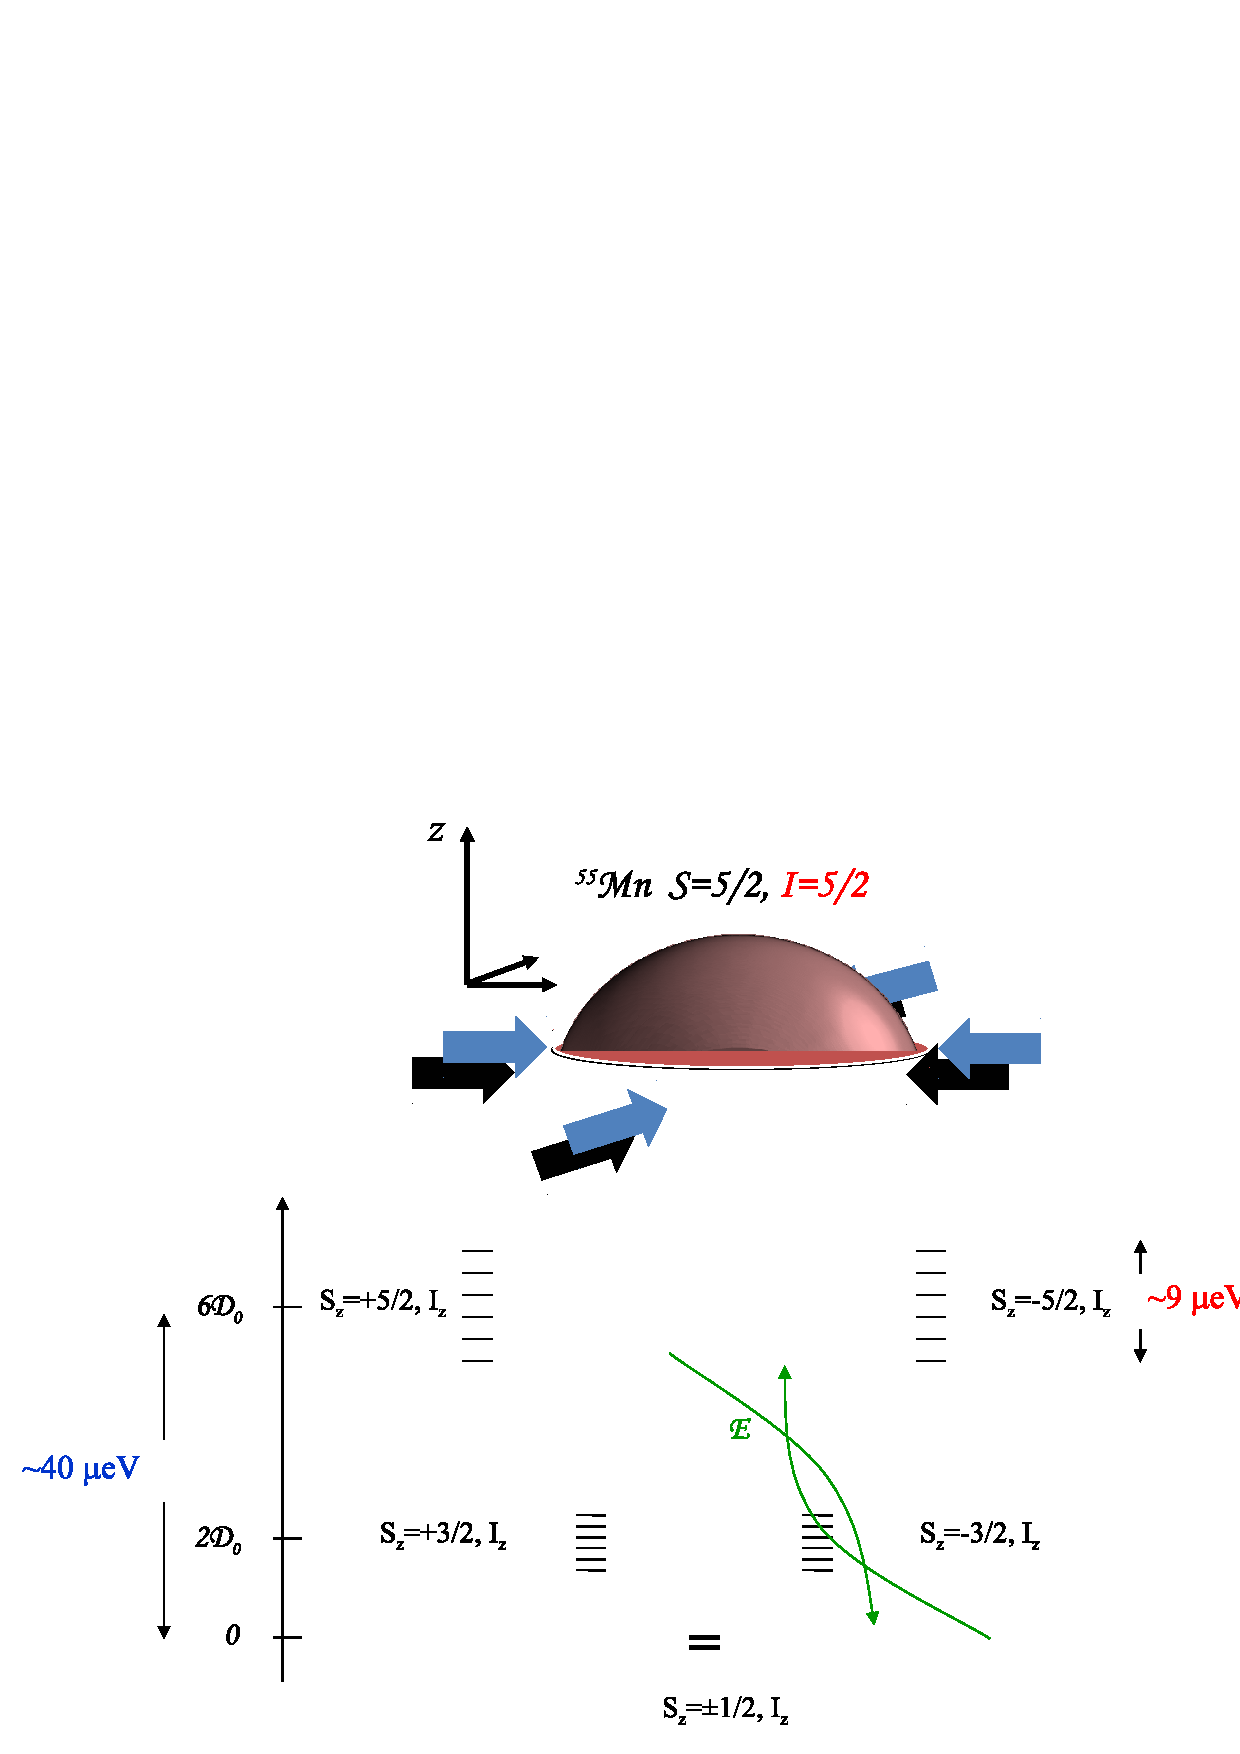
\includegraphics[width=12cm]{Pictures/MnFineStruct.png}
	\end{center}
	\caption{Top: schematic view of a strained QD containing a magnetic atom. Bottom: schema of the fine and hyperfine structure of a Mn atom in a strained II-VI QD. The influence of the magnetic anisotropy $D_0$, the in-plane anisotropy $E$ and the hyperfine interaction ${\cal A}$ are represented.}
	\label{MnFineHyperfines}
	\end{figure}
	
	To describe in detail the spin energy levels of a Mn atom, one has also to consider its nuclear spin is $I = \frac{5}{2}$ for all its isotopes. This nuclear spin couples to the $3d$ electrons via the hyperfine interaction. The whole hamiltonian of an electronic spin coupled to the nuclear spin of a Mn atom in a strained layer grow along [001] axis is known from electron paramagnetic resonance in CdTe/ZnTe superlattices~\cite{StrainedMn} and reads:
	\begin{align}
	\label{Mnalone}
		\begin{array}{rll}
			{\cal H}_{Mn} &=& {\cal A}\mathbf{I}.\mathbf{S} \\
							& & +\dfrac{1}{6}a (S_x^4 + S_y^4 + S_z^4 - \dfrac{1}{5}S(S+1)(3S^2+3S-1)) \\
							& & + D_0 (S_z^2 - \dfrac{1}{3}S(S+1)) + E(S_x^2 - S_y^2)
		\end{array}
	\end{align}
	
	The first term is the hyperfine interaction between the Mn nuclear spin $\mathbf{I}$ and its $5d$ electrons spin $\mathbf{S}$, coupling two consecutive Mn spin states through an electron-nuclei flip flop. The hyperfine constant of the Mn was found to be ${\cal A} \approx 0.71$ $\mu$eV~\cite{MnSpinLatticeCoeff}. The second term results from the crystal cubic symmetry and mixes different $S_z$ of the Mn spin. According to ref.~\cite{MnSpinLatticeCoeff}, $a = 0.32$ $\mu$eV.
	
	The last line contains terms linked to the strain state at the Mn position: the magnetic anisotropy caused by bi-axial strain $D_0$ and the anisotropy of strain in the $xy$ plane $E$. Because of the partial relaxation of strain in the self-assembled QD we used, the value of $D_0$ may vary between 0 $\mu$eV for a strain-free QD, to 12 $\mu$eV for a fully strain CdTe layer matched on ZnTe. Typical values around 7 $\mu$eV are usually observed in CdTe/ZnTe QDs~\cite{MnResSpinDyn,GorycaPrecession}, leading to the 40 $\mu$eV splitting presented on Fig.~\ref{MnFineHyperfines}.
	
	An anisotropy of the strain in the QD plane can induce a mixing between different $S_z$ through the anisotropic crystal field parameter $E$. It coupled two values of $S_z$ separated by two units of spin. In the absence of magnetic anisotropy ($D_0 \simeq 0$), both the anisotropy of strain and the hyperfine structure prevent the optical pumping of the Mn spin at zero magnetic field.

		\subsection{Cr atom in II-VI semiconductor\label{CrSemiCon}}
	
%		As presented in Sec.~\ref{CrDMS}, the Chromium is included in CdTe as Cr$^{2+}$. This isotope has an electronic spin $S = 2$, an orbital momentum $L = 2$ and \emph{no nuclear spin}. Therefore, Cr presents in our sample no hyperfine structure. However, the non-nul orbital momentum shows that it presents a strong coupling to strain. The fine structure will the be of importance in the study of this atom.
		
%	\begin{figure}[h!]
%		\label{Jahn-Teller}
%		\begin{center}
%			\includegraphics[width=10cm]{../FillingPicture.png}
%		\end{center}
%		\caption{Atomic configuration in Jahn-Teller effect + three minima}
%	\end{figure}

		Cr atoms are incorporated into II-VI semiconductors as Cr$^{2+}$ ions on cation sites forming a deep impurity level. 90\% of Cr isotopes presents \emph{no nuclear spin}, meaning we do not have to consider their hyperfine structure. The ground state of a free Cr$^{2+}$ is $^{5}$D with the orbital quantum number L=2 and a spin S=2 yielding a 25-fold degeneracy. In the crystal field of T$_{d}$ symmetry of the tetrahedral cation site in zinc-blende crystal, the degeneracy is partially lifted (see Fig.~\ref{CrinIIVI}): the $^{5}$D term splits into 15-fold degenerate orbital triplet $^{5}$T$_{2}$ and 10-fold degenerate orbital doublet $^{5}$E, separated by a gap $\Delta \approx 0.5$ eV. As in the case of Mn, this transition introduce a path for non-radiative recombination and can kill the luminescence of the host semiconductor. We have then to keep the Cr concentration low in order for this transition to not become the main recombination path.
		
	The Jahn-Teller distortion further reduces the symmetry to D$_{2d}$ and leads to a splitting of the $^{5}$T$_{2}$ ground state into a 5-fold degenerate $^{5}$B$_{2}$ orbital singlet and a $^{5}$E orbital doublet .

		The ground state orbital singlet $^{5}$B$_{2}$ is further split by the spin-orbit interaction. In a strain free crystal, it was found that the ground state splitting can be described by the spin effective Hamiltonian~\cite{EPRCr}:
		\begin{align}
			\label{exchange}
			{\cal H}_{Cr,CF}=D_0S_z^2+\frac{1}{180}F[35S_z^2-30S(S+1)S_z^2+25S_z^2]+\frac{1}{6}a[S_1^4+S_2^4+S_3^4]
		\end{align}
with the Cr spin $S=2$ and $|D_0|\gg|a|$, $|F|$. In the following, we will use $a=0$ and $F=0$. The x, y, z principal axes were found to coincide with the cubic axes (1,2,3) giving rise to three identical sites, each given by \ref{exchange} but with the z axis of each along a different cubic axis (1,2,3). A value of $D_0\approx+30$ $\mu$eV was estimated from Electron Paramagnetic Resonance (EPR) measurements in highly diluted bulk (Cd,Cr)Te~\cite{EPRCr}.

		\begin{figure}[hbt]
			\label{CrinIIVI}
			\begin{center}
				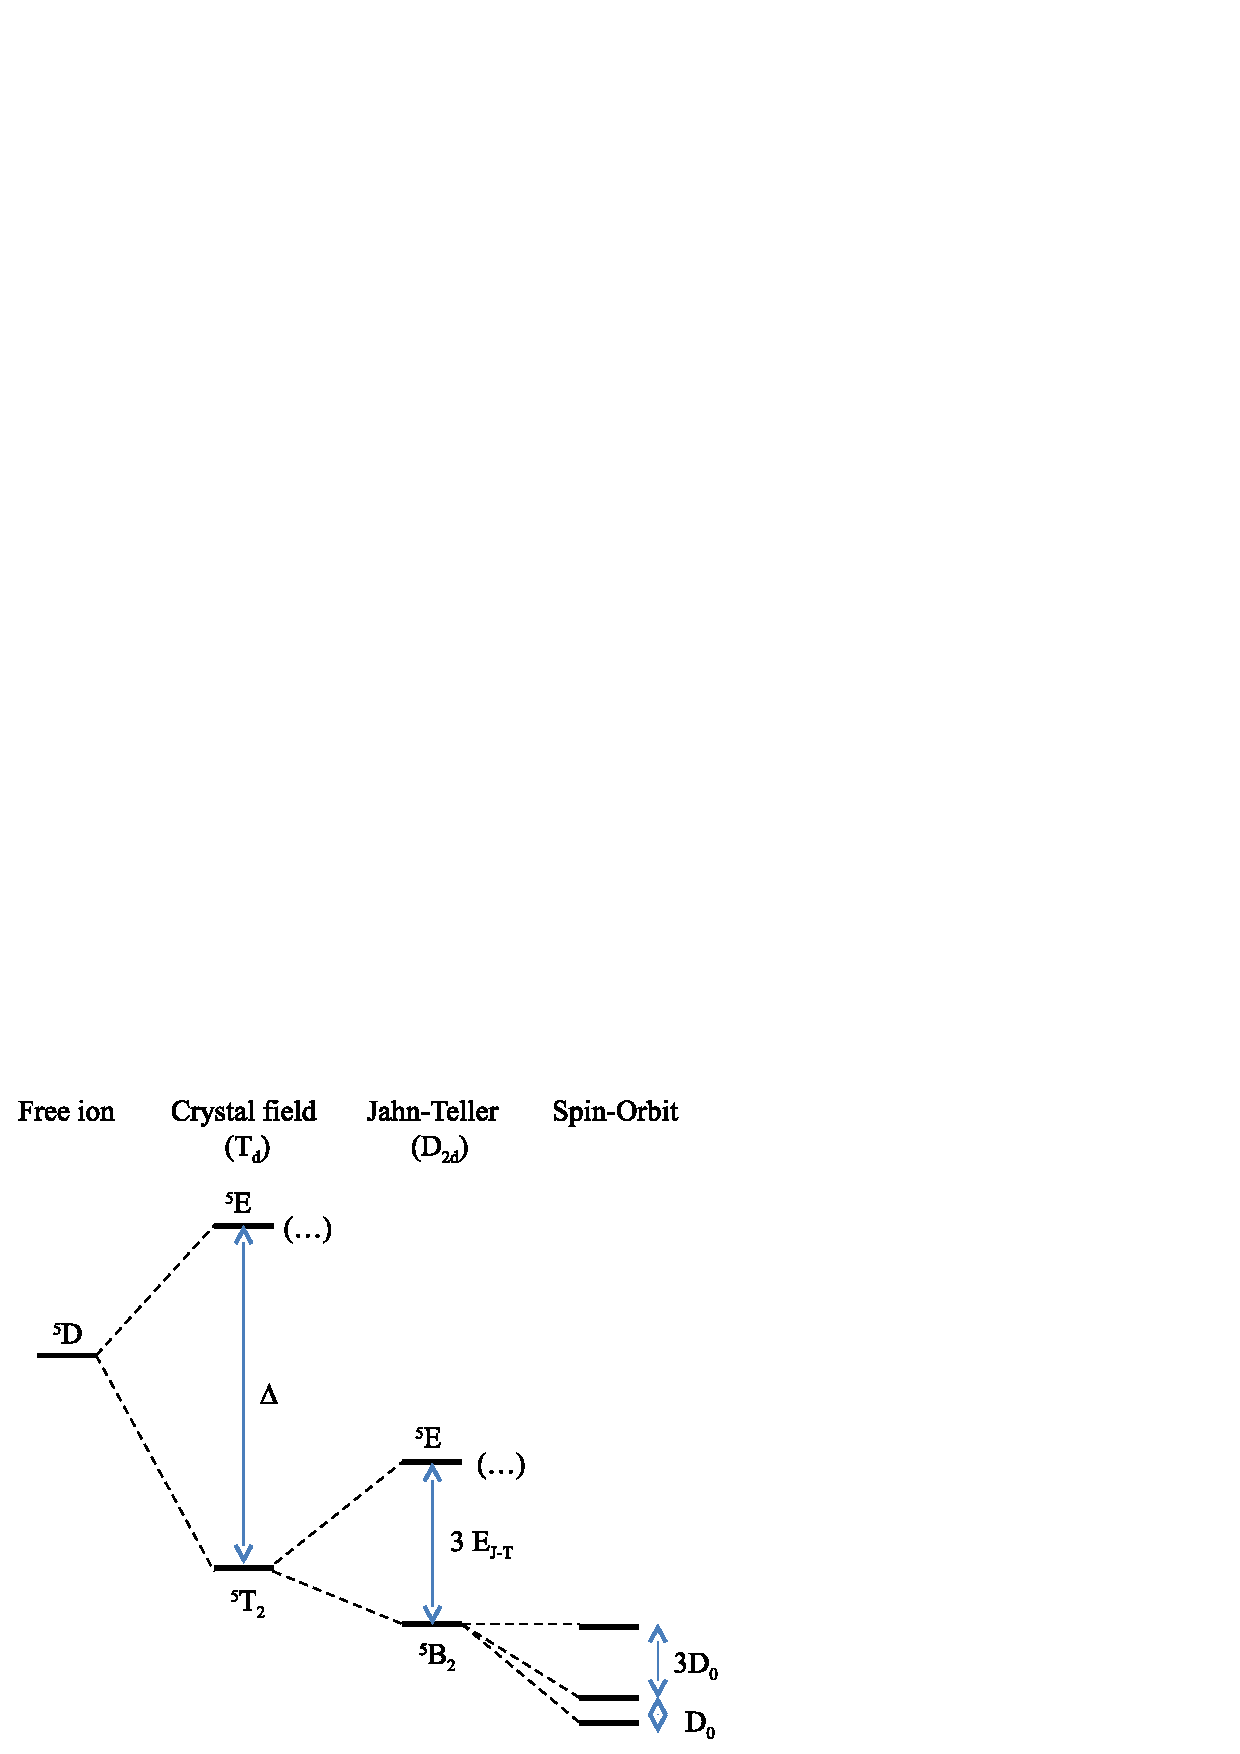
\includegraphics[width=10cm]{Pictures/CrinIIVI.png}
			\end{center}
			\caption{Schema of the energy level splitting of Cr$^{2+}$ at a tetragonal site (T$_d$ symmetry) with a crystal field parameter $\Delta$, a Jahn-Teller energy $E_{J-T}$ and a spin-orbit level spacing $D_0$.}
		\end{figure}
		
		Static biaxial compressive strain in the (001) plane, as observed in self-assembled quantum dots, reduces the symmetry to D$_{2d}$ and destabilize the Cr $3d$ orbitals $d_{xz}$ and $d_{yz}$ having an electron density pointing along the $[$001$]$ axis ($z$ axis). The Cr ground state is then a 5-fold degenerated orbital singlet formed from the $d_{xy}$ orbital. It corresponds to the Jahn-Teller ground state with a tetragonal distortion along the $[$001$]$ axis~\cite{DefPonctSemiCon}.

		An applied stress will also  influence the Cr spin fine structure splitting through the modification of the crystal field and the spin-orbit interaction~\cite{EPRCr}. For an arbitrary strain tensor, the general form of the Cr ground state spin effective Hamiltonian is
		\begin{align}
		\label{FullCrHamil}
			{\cal H}_{Cr,\varepsilon} = c_1 e_A S_{\theta} + c_2 e_{\theta} S_{\theta} + c_3 e_{\epsilon} S_{\epsilon} + c_4e_{\zeta} S_{\zeta} + c_5(e_{\xi} S_{\xi} + e_{\eta} S_{\eta})
		\end{align}
with $S_i$ defined as:
		\begin{align}
			\begin{array}{rl}
			\label{Svalues}
				S_{\theta} &= S_{z}^2  -\dfrac{1}{2} [S_{x}^2 + S_{y}^2] \\
				S_{\epsilon} &= \dfrac{1}{2} \sqrt{3} [S_{x}^2 - S_{y}^2] \\
				S_{\xi} &= S_{y} S_{z} + S_{z} S_{y} \\
				S_{\eta} & = S_{x} S_{z} + S_{z} S_{x} \\
				S_{\zeta} &=S_{x} S_{y} + S_{y} S_{x}
			\end{array}
		\end{align}
and $e_i$ defined similarly as:
		\begin{align}
			\begin{array}{rl}
			\label{evalues}
				e_{\theta} &= \varepsilon_{zz} - \dfrac{1}{2} [\varepsilon_{xx} + \varepsilon_{yy}] \\
				e_{\epsilon} &= \dfrac{1}{2} \sqrt{3}[\varepsilon_{xx} - \varepsilon_{yy}] \\
				e_{\xi} &= \varepsilon_{yz} + \varepsilon_{zy} \\
				e_{\eta} &= \varepsilon_{xz} + \varepsilon_{zx} \\
				e_{\zeta} &= \varepsilon_{xy} + \varepsilon_{yx} \\
				e_A &= \varepsilon_{xx} + \varepsilon_{yy} + \varepsilon_{zz}			
			\end{array}
		\end{align}

		As shown in Sec.~\ref{BPSec}, we can write for a flat self-assembled quantum dot with dominant large biaxial strain:
		\begin{align*}
			\varepsilon_{xx} = \varepsilon_{yy} = \varepsilon_{\parallel} \\
			\varepsilon_{zz}=-2\frac{C_{11}}{C_{12}}\varepsilon_{\parallel}
		\end{align*}
where C$_{11}\approx$ 5.4 10$^{10}$ Pa and C$_{12}\approx$ 3.7 10$^{10}$ Pa are the elastic constants of CdTe~\cite{CdTeElConst}. For this strain configuration, the Cr fine structure is controlled by the spin-lattice coupling coefficients $c_1$ (symmetric coefficient) and $c_2$ (tetragonal coefficients). Strain-coupling coefficients estimated from EPR measurements in bulk Cr doped CdTe are listed in table \ref{StrCouplCoef}.

		\begin{table}[htb] \centering
			\caption{Values for spin to strain coupling coefficients of Cr in bulk CdTe (in $meV$) extracted from ref.~\cite{EPRCr}.\label{StrCouplCoef}}
			\renewcommand{\arraystretch}{1.0}
			\begin{tabular}{ccccc}
				\hline\hline
				$c_{1}$ & $c_{2}$ & $c_{3}$  & $c_{4}$  & $c_{5}$ \\
				-0.25$\pm$2 & +4.9 $\pm$2& -1.25$\pm$0.5 & +4.9$\pm$2 & +3.7$\pm$1.25 \\
				\hline\hline
			\end{tabular}
		\end{table}

		We can now simplify the hamiltonian \ref{FullCrHamil}, first reducing it to the active term in our case:
		\begin{align*}
			{\cal H}_{Cr,\varepsilon} &= c_1 e_A S_{\theta} + c_2 e_{\theta} S_{\theta}
		\end{align*}
Replacing now $e_A$, $e_{\theta}$ and $S_{\theta}$ by their value given in \ref{Svalues} and \ref{evalues}, and using the equalities given in Sec.~\ref{BPSec}, we can rewrite the strain controlled part of the spin Hamiltonian as ${\cal H}_{Cr,\varepsilon}$, depending only on $\varepsilon_{\parallel}$:
		\begin{align}
			\begin{array}{rlcc}
			\label{HamilD0}
				{\cal H}_{Cr,\varepsilon_{\parallel}} &=& \underbrace{\dfrac{3}{2}\varepsilon_{\parallel}[2c_1(1-\dfrac{C_{12}}{C_{11}})-c_2(1+2\dfrac{C_{12}}{C_{11}})]} & S_z^2 \\
													&=& D_0 & S_z^2
			\end{array}
		\end{align}
where we can estimate $D_0\approx 1\pm0.6$ meV from the values of the spin-strain coupling coefficients in CdTe (table \ref{StrCouplCoef}). This is about 100 times stronger than the value found in Mn QDs, as stated on Sec.~\ref{MnSemiCon}.
%\newline
%{\Large FIND A WAY TO REFORMULATE}\newline
One should note the QDs could be partially relaxed and may contain a significant amount of Zn. This could significantly change the spin-strain coupling coefficients of the Cr atom.
%We were not able to find spin to strain coupling coefficients for Cr in ZnTe and (Cd,Zn)Te alloy in literature. A value of D$_0\approx$+280 $\mu$eV, much larger than for CdTe, was however estimated in strain-free Cr-doped bulk ZnTe~\cite{EPRCr}. Larger spin-strain coupling coefficients could than expected for Cr in ZnTe and (Cd,Zn)Te alloys.

		An anisotropy of the strain in the quantum dot plane (001) with principal axis along $[$010$]$ or $[$100$]$ axes ($\varepsilon_{xx}\neq\varepsilon_{yy}$ and $\varepsilon_{xy} = \varepsilon_{yx}=0$) would affect the Cr fine structure through the tetragonal coefficient $c_3$. This coupling can be described by an additional term in the spin-strain Hamiltonian
		\begin{align}
			\begin{array}{rlcc}
			\label{HamilE}
				{\cal H}_{Cr,\varepsilon_{\perp}} &=& \underbrace{\dfrac{3}{4} c_3 (\varepsilon_{xx}-\varepsilon_{yy})} & (S_x^2 - S_y^2) \\
												&=& E & (S_x^2 - S_y^2)
			\end{array}
		\end{align}

		This anisotropy term $E$ couples Cr spin states separated by two units and in particular $S_z$=+1 to $S_z$=-1 which are initially degenerated. It could be exploited to induce a large strain mediated coherent coupling between a mechanical oscillator and the Cr spin~\cite{SpinOsciCoupl}.
		
		We can now group \ref{HamilD0} and \ref{HamilE} in order to write the complete hamiltonian of an isolated Cr in a CdTe/ZnTe QD with anisotropic strains :
		\begin{align}
			\label{Cralone}
			{\cal H}_{Cr,\varepsilon} = D_0 S_z^2 + E(S_x^2 - S_y^2)
		\end{align}
		
		This large sensitivity of the Cr spin to local strains makes the Cr a particularly interesting qubit for the development of hybrid spin-mechanical systems~\cite{CouplingNVOscill,LafuenteStrainMn,QuantSpinTrasducer}.
	
	
	\section{The X-Mn system\label{XMn}}
	
	In order to illustrate the concepts explained in this chapter, we will present a quick study of a well known system: the exciton coupled to a single Manganese atom. In order to simplify the study, let's consider a QD containing a single Mn atom with no shape or strain anisotropy. When an exciton is injected in the QD, it will interact with the magnetic atom spin in addition to the hole-electron interaction already taking place for an exciton. The hamiltonian of the system reads:
	\begin{align}
		\label{HXMn}
		{\cal H}_{XMn} = {\cal H}_{eh} + {\cal H}_{eMn} + {\cal H}_{hMn}
	\end{align}
We use in this part the heavy-hole approximation, ignoring the effect of the non-diagonal term of the band hamiltonian.

	\begin{figure}[h!]
	\begin{center}
		\includegraphics[width=11cm]{Pictures/XMn-Exp.eps}
	\end{center}
	\caption{Photoluminescence of the X, X$^-$ and X$^2$ complex for (a) a QD with no magnetic atom and (b) a QD containing a single Mn atom.}
	\label{MnSpectra}
	\end{figure}

	In the heavy hole subspace, in the $\sigma_z$, $j_z$, $S_z$ basis, all the hamiltonians describing an interaction with the hole are diagonal. Therefore, the only non-diagonal element in the hamiltonian~\ref{HXMn} describe electron-Mn spin-flips. The hole having no part in this interaction, those spin-flips couple a bright state to a dark state, separated by $\delta_0$, as defined in Sec.~\ref{ehExch}. The strength of this interaction is of the same magnitude as $I_{eMn}$, found to be in the 100 $\mu$eV range in our quantum dots~\cite{DynhMn}. Since distance between the bright and dark states is about one order of magnitude higher than the strength of the interaction, we neglect it.
	
	\begin{figure}[h!]
	\begin{center}
		\includegraphics[width=12cm]{Pictures/MnEnLvl.png}
	\end{center}
	\caption{Energy level of the ground state and the exciton in a Mn-doped QD. The levels are sketched as a function of the Mn spin $S_z$. Dark states are represented in grey. Optical transitions from the bright states of the Mn complex results in six-line PL spectra, such as in Fig.~\ref{MnSpectra}.}
	\label{MnLevel}
	\end{figure}
	
	We can now consider the hamiltonian~\ref{HXMn} to be diagonal. The interaction of the Mn spin with electron is ferromagnetic with $I_{eMn} \simeq -100$ $\mu$eV, while its interaction with the hole is anti-ferromagnetic with $I_{hMn} \simeq 250$ $\mu$eV.  The carriers act on the Mn spin as an effective magnetic field oriented along the growth axis. This lift the degeneracy of the Mn spins in a sextuplet. For the bright exciton, with anti-parallel electron and hole spins, the splitting is the widest. Each Mn spin state is separated from the closest one by $\frac{1}{2}(3I_{hMn} - I_{eMn})$, for a total energy span of $\frac{5}{2}(3I_{hMn} - I_{eMn})$. For the dark exciton states, each of them are separated from the closest one by $\frac{1}{2}(3I_{hMn} + I_{eMn})$, for total energy span of $\frac{5}{2}(3I_{hMn} + I_{eMn})$. The bright and dark excitons are split by the electron-hole exchange interaction is given by $\delta_0 = -\frac{3}{2}I_{eh} \approx 1$ meV, with $I_{eh} \simeq -750$ $\mu$eV. All these splitting are a lot larger than the one induced by the crystal field and the hyperfine interaction.
	
	One can note that the system is symmetric under inversion of the quantization axis $z$. Excitons with opposed spins coupled to opposed Mn spins will then be degenerated. For instance, $|S_z = \frac{5}{2}, X_z = -1\rangle$ share the same energy level as $|S_z = -\frac{5}{2}, X_z = +1\rangle$. The whole energy level structure is summarize in Fig.~\ref{MnLevel}.
	
	The fundamental state of the QD is an isolated Mn atom in the dot. In our QDs, we usually find $D_0 \simeq 7$ $\mu$eV~\cite{MnResSpinDyn,GorycaPrecession}, negligible compared to the exciton-Mn interactions. Since the other fine structure parameters of the Mn are weaker than $D_0$, we can neglect their contribution to the spectra. Therefore, the fundamental state of the QD is six time degenerated. The recombination does not affect the Mn spin. Each emission line is thus the superposition of two optical transitions with opposed circular polarization (recombination of an exciton $X_z = \pm1$). In a given polarization, each line corresponds then to a single Mn spin: the spectra is a picture of the statistic state of the Mn spin when the exciton recombines.

%	To go more in details in the understanding of the system, we should also include the effect of the short range interaction and the VBM. We saw that the short range e-h exchange couple bright exciton states together. In Mn-doped QD, this translates to a coupling between bright states associated with the same Mn spin projection. However, one can see on Fig.~\ref{MnLevel}, for most X-Mn levels, two opposite-spin excitons coupled to the same Mn spin are far from each other in energy. Therefore, this coupling mainly  apply to the level coupled to $|S_z = \pm\frac{1}{2}\rangle$, only slightly splitted by  the exciton-Mn exchange interaction.
	
	This simple model is however incomplete. More thorough investigation of the system were done in \cite{YoanTh}. The effects of the VBM, and the strain and shape anisotropy on the system was studied in \cite{DELum}. A complete study of the spin dynamics of the system was also done by Claire Le Gall in her PhD thesis~\cite{ClaireTh}.
	
\printbibliography

\end{document}